%%%%%%%%%%%%%%%%%%%%%%%%%%%%%%%%%%%%%%%%%
% Important note:
% Chapter heading images should have a 2:1 width:height ratio,
% e.g. 920px width and 460px height.
%
%%%%%%%%%%%%%%%%%%%%%%%%%%%%%%%%%%%%%%%%%


%----------------------------------------------------------------------------------------
%	PACKAGES AND OTHER DOCUMENT CONFIGURATIONS
%----------------------------------------------------------------------------------------

\documentclass[openany,11pt,fleqn]{book} % Default font size and left-justified equations

\usepackage[top=3cm,bottom=3cm,left=3.2cm,right=3.2cm,headsep=10pt,letterpaper]{geometry} % Page margins

\usepackage{xcolor} % Required for specifying colors by name
\definecolor{ocre}{RGB}{52,177,201} % Define the orange color used for highlighting throughout the book

% Font Settings
\usepackage{avant} % Use the Avantgarde font for headings
%\usepackage{times} % Use the Times font for headings
\usepackage{mathptmx} % Use the Adobe Times Roman as the default text font together with math symbols from the Sym­bol, Chancery and Com­puter Modern fonts
\usepackage{microtype} % Slightly tweak font spacing for aesthetics
\usepackage[utf8]{inputenc} % Required for including letters with accents
\usepackage[T1]{fontenc} % Use 8-bit encoding that has 256 glyphs
\usepackage{amsthm}

\usepackage{subcaption}

\usepackage{mathtools}

\usepackage{minted}

\usepackage{tikz}
\usepackage{pgfplots}
\usepgfplotslibrary{fillbetween}
\usepackage{multirow}
\usepackage{array}
\usetikzlibrary{arrows.meta, positioning, calc, trees, shapes, decorations, matrix, fit}

% Bibliography
\usepackage[style=alphabetic,sorting=nyt,sortcites=true,autopunct=true,babel=hyphen,hyperref=true,abbreviate=false,backref=true,backend=biber]{biblatex}
\addbibresource{bibliography.bib} % BibTeX bibliography file
\defbibheading{bibempty}{}
\usepackage{float}


%----------------------------------------------------------------------------------------
%	VARIOUS REQUIRED PACKAGES
%----------------------------------------------------------------------------------------

\usepackage{titlesec} % Allows customization of titles

\usepackage{graphicx} % Required for including pictures
\graphicspath{{Pictures/}} % Specifies the directory where pictures are stored
% \graphicspath{{Plots/}}
\usepackage{lipsum} % Inserts dummy text

\usepackage{tikz} % Required for drawing custom shapes

\usepackage[english]{babel} % English language/hyphenation

\usepackage{enumitem} % Customize lists
\setlist{nolistsep} % Reduce spacing between bullet points and numbered lists

\usepackage{booktabs} % Required for nicer horizontal rules in tables

\usepackage{eso-pic} % Required for specifying an image background in the title page

%----------------------------------------------------------------------------------------
%	MAIN TABLE OF CONTENTS
%----------------------------------------------------------------------------------------

\usepackage{titletoc} % Required for manipulating the table of contents

\contentsmargin{0cm} % Removes the default margin
% Chapter text styling
\titlecontents{chapter}[1.25cm] % Indentation
{\addvspace{15pt}\large\sffamily\bfseries} % Spacing and font options for chapters
{\color{ocre!60}\contentslabel[\thecontentslabel]{2cm}\color{ocre}} % Chapter number
{}  
{\color{ocre!60}\normalsize\sffamily\bfseries\;\titlerule*[.5pc]{.}\;\thecontentspage} % Page number
% Section text styling
\titlecontents{section}[1.25cm] % Indentation
{\addvspace{5pt}\sffamily\bfseries} % Spacing and font options for sections
{\contentslabel[\thecontentslabel]{1.25cm}} % Section number
{}
{\sffamily\hfill\color{black}\thecontentspage} % Page number
[]
% Subsection text styling
\titlecontents{subsection}[1.25cm] % Indentation
{\addvspace{1pt}\sffamily\small} % Spacing and font options for subsections
{\contentslabel[\thecontentslabel]{1.25cm}} % Subsection number
{}
{\sffamily\;\titlerule*[.5pc]{.}\;\thecontentspage} % Page number
[] 

%----------------------------------------------------------------------------------------
%	MINI TABLE OF CONTENTS IN CHAPTER HEADS
%----------------------------------------------------------------------------------------

% Section text styling
\titlecontents{lsection}[0em] % Indendating
{\footnotesize\sffamily} % Font settings
{}
{}
{}

% Subsection text styling
\titlecontents{lsubsection}[.5em] % Indentation
{\normalfont\footnotesize\sffamily} % Font settings
{}
{}
{}
 
%----------------------------------------------------------------------------------------
%	PAGE HEADERS
%----------------------------------------------------------------------------------------

\usepackage{fancyhdr} % Required for header and footer configuration

\pagestyle{fancy}
\renewcommand{\chaptermark}[1]{\markboth{\sffamily\normalsize\bfseries\chaptername\ \thechapter.\ #1}{}} % Chapter text font settings
\renewcommand{\sectionmark}[1]{\markright{\sffamily\normalsize\thesection\hspace{5pt}#1}{}} % Section text font settings
\fancyhf{} \fancyhead[LE,RO]{\sffamily\normalsize\thepage} % Font setting for the page number in the header
\fancyhead[LO]{\rightmark} % Print the nearest section name on the left side of odd pages
\fancyhead[RE]{\leftmark} % Print the current chapter name on the right side of even pages
\renewcommand{\headrulewidth}{0.5pt} % Width of the rule under the header
\addtolength{\headheight}{2.5pt} % Increase the spacing around the header slightly
\renewcommand{\footrulewidth}{0pt} % Removes the rule in the footer
\fancypagestyle{plain}{\fancyhead{}\renewcommand{\headrulewidth}{0pt}} % Style for when a plain pagestyle is specified

% Removes the header from odd empty pages at the end of chapters
\makeatletter
\renewcommand{\cleardoublepage}{
\clearpage\ifodd\c@page\else
\hbox{}
\vspace*{\fill}
\thispagestyle{empty}
\newpage
\fi}

%----------------------------------------------------------------------------------------
%	THEOREM STYLES
%----------------------------------------------------------------------------------------

\usepackage{amsmath,amsfonts,amssymb,amsthm} % For math equations, theorems, symbols, etc

\newcommand{\intoo}[2]{\mathopen{]}#1\,;#2\mathclose{[}}
\newcommand{\ud}{\mathop{\mathrm{{}d}}\mathopen{}}
\newcommand{\intff}[2]{\mathopen{[}#1\,;#2\mathclose{]}}
\newtheorem{notation}{Notation}[chapter]

%%%%%%%%%%%%%%%%%%%%%%%%%%%%%%%%%%%%%%%%%%%%%%%%%%%%%%%%%%%%%%%%%%%%%%%%%%%
%%%%%%%%%%%%%%%%%%%% dedicated to boxed/framed environements %%%%%%%%%%%%%%
%%%%%%%%%%%%%%%%%%%%%%%%%%%%%%%%%%%%%%%%%%%%%%%%%%%%%%%%%%%%%%%%%%%%%%%%%%%
\newtheoremstyle{ocrenumbox}% % Theorem style name
{0pt}% Space above
{0pt}% Space below
{\normalfont}% % Body font
{}% Indent amount
{\small\bf\sffamily\color{ocre}}% % Theorem head font
{\;}% Punctuation after theorem head
{0.25em}% Space after theorem head
{\small\sffamily\color{ocre}\thmname{#1}\nobreakspace\thmnumber{\@ifnotempty{#1}{}\@upn{#2}}% Theorem text (e.g. Theorem 2.1)
\thmnote{\nobreakspace\the\thm@notefont\sffamily\bfseries\color{black}---\nobreakspace#3.}} % Optional theorem note
\renewcommand{\qedsymbol}{$\blacksquare$}% Optional qed square

\newtheoremstyle{blacknumex}% Theorem style name
{5pt}% Space above
{5pt}% Space below
{\normalfont}% Body font
{} % Indent amount
{\small\bf\sffamily}% Theorem head font
{\;}% Punctuation after theorem head
{0.25em}% Space after theorem head
{\small\sffamily{\tiny\ensuremath{\blacksquare}}\nobreakspace\thmname{#1}\nobreakspace\thmnumber{\@ifnotempty{#1}{}\@upn{#2}}% Theorem text (e.g. Theorem 2.1)
\thmnote{\nobreakspace\the\thm@notefont\sffamily\bfseries---\nobreakspace#3.}}% Optional theorem note

\newtheoremstyle{blacknumbox} % Theorem style name
{0pt}% Space above
{0pt}% Space below
{\normalfont}% Body font
{}% Indent amount
{\small\bf\sffamily}% Theorem head font
{\;}% Punctuation after theorem head
{0.25em}% Space after theorem head
{\small\sffamily\thmname{#1}\nobreakspace\thmnumber{\@ifnotempty{#1}{}\@upn{#2}}% Theorem text (e.g. Theorem 2.1)
\thmnote{\nobreakspace\the\thm@notefont\sffamily\bfseries---\nobreakspace#3.}}% Optional theorem note

%%%%%%%%%%%%%%%%%%%%%%%%%%%%%%%%%%%%%%%%%%%%%%%%%%%%%%%%%%%%%%%%%%%%%%%%%%%
%%%%%%%%%%%%% dedicated to non-boxed/non-framed environements %%%%%%%%%%%%%
%%%%%%%%%%%%%%%%%%%%%%%%%%%%%%%%%%%%%%%%%%%%%%%%%%%%%%%%%%%%%%%%%%%%%%%%%%%
\newtheoremstyle{ocrenum}% % Theorem style name
{5pt}% Space above
{5pt}% Space below
{\normalfont}% % Body font
{}% Indent amount
{\small\bf\sffamily\color{ocre}}% % Theorem head font
{\;}% Punctuation after theorem head
{0.25em}% Space after theorem head
{\small\sffamily\color{ocre}\thmname{#1}\nobreakspace\thmnumber{\@ifnotempty{#1}{}\@upn{#2}}% Theorem text (e.g. Theorem 2.1)
\thmnote{\nobreakspace\the\thm@notefont\sffamily\bfseries\color{black}---\nobreakspace#3.}} % Optional theorem note
\renewcommand{\qedsymbol}{$\blacksquare$}% Optional qed square
\makeatother

% Defines the theorem text style for each type of theorem to one of the three styles above
\newcounter{dummy} 
\numberwithin{dummy}{section}
\theoremstyle{ocrenumbox}


\newtheorem{theoremeT}[dummy]{Theorem}
\newtheorem{lemma}[dummy]{Lemma}
\newtheorem{observation}[dummy]{Observation}
\newtheorem{proposition}[dummy]{Proposition}
% \newtheorem{definition}[dummy]{Definition}
\newtheorem{claim}[dummy]{Claim}
\newtheorem{fact}[dummy]{Fact}
\newtheorem{assumption}[dummy]{Assumption}

\newtheorem{problem}{Problem}[chapter]
% \newtheorem{exercise}{Exercise}[chapter]
\theoremstyle{blacknumex}
\newtheorem{exampleT}{Example}[chapter]
\theoremstyle{blacknumbox}
\newtheorem{vocabulary}{Vocabulary}[chapter]
\newtheorem{definitionT}{Definition}[section]
\newtheorem{corollaryT}[dummy]{Corollary}
\theoremstyle{ocrenum}



%----------------------------------------------------------------------------------------
%	DEFINITION OF COLORED BOXES
%----------------------------------------------------------------------------------------

\RequirePackage[framemethod=default]{mdframed} % Required for creating the theorem, definition, exercise and corollary boxes

% Theorem box
\newmdenv[skipabove=7pt,
skipbelow=7pt,
backgroundcolor=black!5,
linecolor=ocre,
innerleftmargin=5pt,
innerrightmargin=5pt,
innertopmargin=5pt,
leftmargin=0cm,
rightmargin=0cm,
innerbottommargin=5pt]{tBox}

% Exercise box	  
\newmdenv[skipabove=7pt,
skipbelow=7pt,
rightline=false,
leftline=true,
topline=false,
bottomline=false,
backgroundcolor=ocre!10,
linecolor=ocre,
innerleftmargin=5pt,
innerrightmargin=5pt,
innertopmargin=5pt,
innerbottommargin=5pt,
leftmargin=0cm,
rightmargin=0cm,
linewidth=4pt]{eBox}	

% Definition box
\newmdenv[skipabove=7pt,
skipbelow=7pt,
rightline=false,
leftline=true,
topline=false,
bottomline=false,
linecolor=ocre,
innerleftmargin=5pt,
innerrightmargin=5pt,
innertopmargin=0pt,
leftmargin=0cm,
rightmargin=0cm,
linewidth=4pt,
innerbottommargin=0pt]{dBox}	

% Corollary box
\newmdenv[skipabove=7pt,
skipbelow=7pt,
rightline=false,
leftline=true,
topline=false,
bottomline=false,
linecolor=gray,
backgroundcolor=black!5,
innerleftmargin=5pt,
innerrightmargin=5pt,
innertopmargin=5pt,
leftmargin=0cm,
rightmargin=0cm,
linewidth=4pt,
innerbottommargin=5pt]{cBox}

% Creates an environment for each type of theorem and assigns it a theorem text style from the "Theorem Styles" section above and a colored box from above
\newenvironment{theorem}{\begin{tBox}\begin{theoremeT}}{\end{theoremeT}\end{tBox}}
\newenvironment{exercise}{\begin{eBox}\begin{exerciseT}}{\hfill{\color{ocre}\tiny\ensuremath{\blacksquare}}\end{exerciseT}\end{eBox}}				  
\newenvironment{definition}{\begin{dBox}\begin{definitionT}}{\end{definitionT}\end{dBox}}	
\newenvironment{example}{\begin{exampleT}}{\hfill{\tiny\ensuremath{\blacksquare}}\end{exampleT}}		
\newenvironment{corollary}{\begin{cBox}\begin{corollaryT}}{\end{corollaryT}\end{cBox}}	

%----------------------------------------------------------------------------------------
%	REMARK ENVIRONMENT
%----------------------------------------------------------------------------------------

\newenvironment{remark}{\par\vspace{10pt}\small % Vertical white space above the remark and smaller font size
\begin{list}{}{
\leftmargin=35pt % Indentation on the left
\rightmargin=25pt}\item\ignorespaces % Indentation on the right
\makebox[-2.5pt]{\begin{tikzpicture}[overlay]
\node[draw=ocre!60,line width=1pt,circle,fill=ocre!25,font=\sffamily\bfseries,inner sep=2pt,outer sep=0pt] at (-15pt,0pt){\textcolor{ocre}{R}};\end{tikzpicture}} % Orange R in a circle
\advance\baselineskip -1pt}{\end{list}\vskip5pt} % Tighter line spacing and white space after remark

%----------------------------------------------------------------------------------------
%	SECTION NUMBERING IN THE MARGIN
%----------------------------------------------------------------------------------------

\makeatletter
\renewcommand{\@seccntformat}[1]{\llap{\textcolor{ocre}{\csname the#1\endcsname}\hspace{1em}}}                    
\renewcommand{\section}{\@startsection{section}{1}{\z@}
{-4ex \@plus -1ex \@minus -.4ex}
{1ex \@plus.2ex }
{\normalfont\large\sffamily\bfseries}}
\renewcommand{\subsection}{\@startsection {subsection}{2}{\z@}
{-3ex \@plus -0.1ex \@minus -.4ex}
{0.5ex \@plus.2ex }
{\normalfont\sffamily\bfseries}}
\renewcommand{\subsubsection}{\@startsection {subsubsection}{3}{\z@}
{-2ex \@plus -0.1ex \@minus -.2ex}
{.2ex \@plus.2ex }
{\normalfont\small\sffamily\bfseries}}                        
\renewcommand\paragraph{\@startsection{paragraph}{4}{\z@}
{-2ex \@plus-.2ex \@minus .2ex}
{.1ex}
{\normalfont\small\sffamily\bfseries}}

%----------------------------------------------------------------------------------------
%	HYPERLINKS IN THE DOCUMENTS
%----------------------------------------------------------------------------------------

% For an unclear reason, the package should be loaded now and not later
\usepackage{hyperref}
\hypersetup{hidelinks,backref=true,pagebackref=true,hyperindex=true,colorlinks=false,breaklinks=true,urlcolor= ocre,bookmarks=true,bookmarksopen=false,pdftitle={Title},pdfauthor={Author}}

%----------------------------------------------------------------------------------------
%	CHAPTER HEADINGS
%----------------------------------------------------------------------------------------

% The set-up below should be (sadly) manually adapted to the overall margin page septup controlled by the geometry package loaded in the main.tex document. It is possible to implement below the dimensions used in the goemetry package (top,bottom,left,right)... TO BE DONE

\newcommand{\thechapterimage}{}
\newcommand{\chapterimage}[1]{\renewcommand{\thechapterimage}{#1}}

% Numbered chapters with mini tableofcontents
\def\thechapter{\arabic{chapter}}
\def\@makechapterhead#1{
\thispagestyle{empty}
{\centering \normalfont\sffamily
\ifnum \c@secnumdepth >\m@ne
\if@mainmatter
\startcontents
\begin{tikzpicture}[remember picture,overlay]
\node at (current page.north west)
{\begin{tikzpicture}[remember picture,overlay]
\node[anchor=north west,inner sep=0pt] at (0,0) {\includegraphics[width=\paperwidth]{\thechapterimage}};
%%%%%%%%%%%%%%%%%%%%%%%%%%%%%%%%%%%%%%%%%%%%%%%%%%%%%%%%%%%%%%%%%%%%%%%%%%%%%%%%%%%%%
% Commenting the 3 lines below removes the small contents box in the chapter heading
%\fill[color=ocre!10!white,opacity=.6] (1cm,0) rectangle (8cm,-7cm);
%\node[anchor=north west] at (1.1cm,.35cm) {\parbox[t][8cm][t]{6.5cm}{\huge\bfseries\flushleft \printcontents{l}{1}{\setcounter{tocdepth}{2}}}};
\draw[anchor=west] (5cm,-9cm) node [rounded corners=20pt,fill=ocre!10!white,text opacity=1,draw=ocre,draw opacity=1,line width=1.5pt,fill opacity=.6,inner sep=12pt]{\Large\sffamily\bfseries\textcolor{black}{\thechapter. #1\strut\makebox[22cm]{}}};
%%%%%%%%%%%%%%%%%%%%%%%%%%%%%%%%%%%%%%%%%%%%%%%%%%%%%%%%%%%%%%%%%%%%%%%%%%%%%%%%%%%%%
\end{tikzpicture}};
\end{tikzpicture}}
\vskip 223pt % Changed to \vskip from \par\vspace*{} bc it was skipping pages for me
\fi
\fi}

% Unnumbered chapters without mini tableofcontents (could be added though) 
\def\@makeschapterhead#1{
\thispagestyle{empty}
{\centering \normalfont\sffamily
\ifnum \c@secnumdepth >\m@ne
\if@mainmatter
\begin{tikzpicture}[remember picture,overlay]
\node at (current page.north west)
{\begin{tikzpicture}[remember picture,overlay]
\node[anchor=north west,inner sep=0pt] at (0,0) {\includegraphics[width=\paperwidth]{\thechapterimage}};
\draw[anchor=west] (5cm,-9cm) node [rounded corners=20pt,fill=ocre!10!white,fill opacity=.6,inner sep=12pt,text opacity=1,draw=ocre,draw opacity=1,line width=1.5pt]{\huge\sffamily\bfseries\textcolor{black}{#1\strut\makebox[22cm]{}}};
\end{tikzpicture}};
\end{tikzpicture}}
\vskip 223pt % Changed to \vskip from \par\vspace*{} bc it was skipping pages for me
\fi
\fi
}
\makeatother % Insert the commands.tex file which contains the majority of the structure behind the template

%----------------------------------------------------------------------------------------
%	Definitions of new commands
%----------------------------------------------------------------------------------------

\newcounter{ttl@toc@default} % Add counter definition

\newcommand{\cvx}{convex}
\thinmuskip=6mu
\medmuskip=8mu plus 4mu minus 6mu
\thickmuskip=10mu plus 10mu
\setlength{\parindent}{0pt} % Remove paragraph indentation
\setlength{\parskip}{0pt} % Remove paragraph skip
\allowdisplaybreaks

\includeonly{
    LECTURE_1/lecture_1.tex,
    LECTURE_2/lecture_2.tex,
    % LECTURE_3/lecture_3.tex,
    % LECTURE_4/lecture_4.tex,
    % LECTURE_5/lecture_5.tex,
    % LECTURE_6/lecture_6.tex
}

\begin{document}

\renewcommand{\thedummy}{\Roman{chapter}.\Roman{section}.\Roman{dummy}}
\renewcommand{\thedefinitionT}{\Roman{chapter}.\Roman{section}.\Roman{definitionT}}
\renewcommand{\theexampleT}{\Roman{chapter}.\Roman{exampleT}}
\renewcommand{\thechapter}{Lecture \Roman{chapter}} % Chapter numbering in Roman numerals
\renewcommand{\thesection}{\Roman{chapter}.\Roman{section}} % Section numbering in Roman numerals
\renewcommand{\thesubsection}{\Roman{chapter}.\Roman{section}.\Roman{subsection}} % Subsection numbering in Roman numerals
\renewcommand{\thetable}{\Roman{chapter}.\Roman{table}}
\renewcommand{\theequation}{\Roman{chapter}.\Roman{equation}}
\renewcommand{\theproblem}{\Roman{problem}}


%----------------------------------------------------------------------------------------
%	TITLE PAGE
%----------------------------------------------------------------------------------------

\begingroup
\thispagestyle{empty}
\AddToShipoutPicture*{\put(0,0){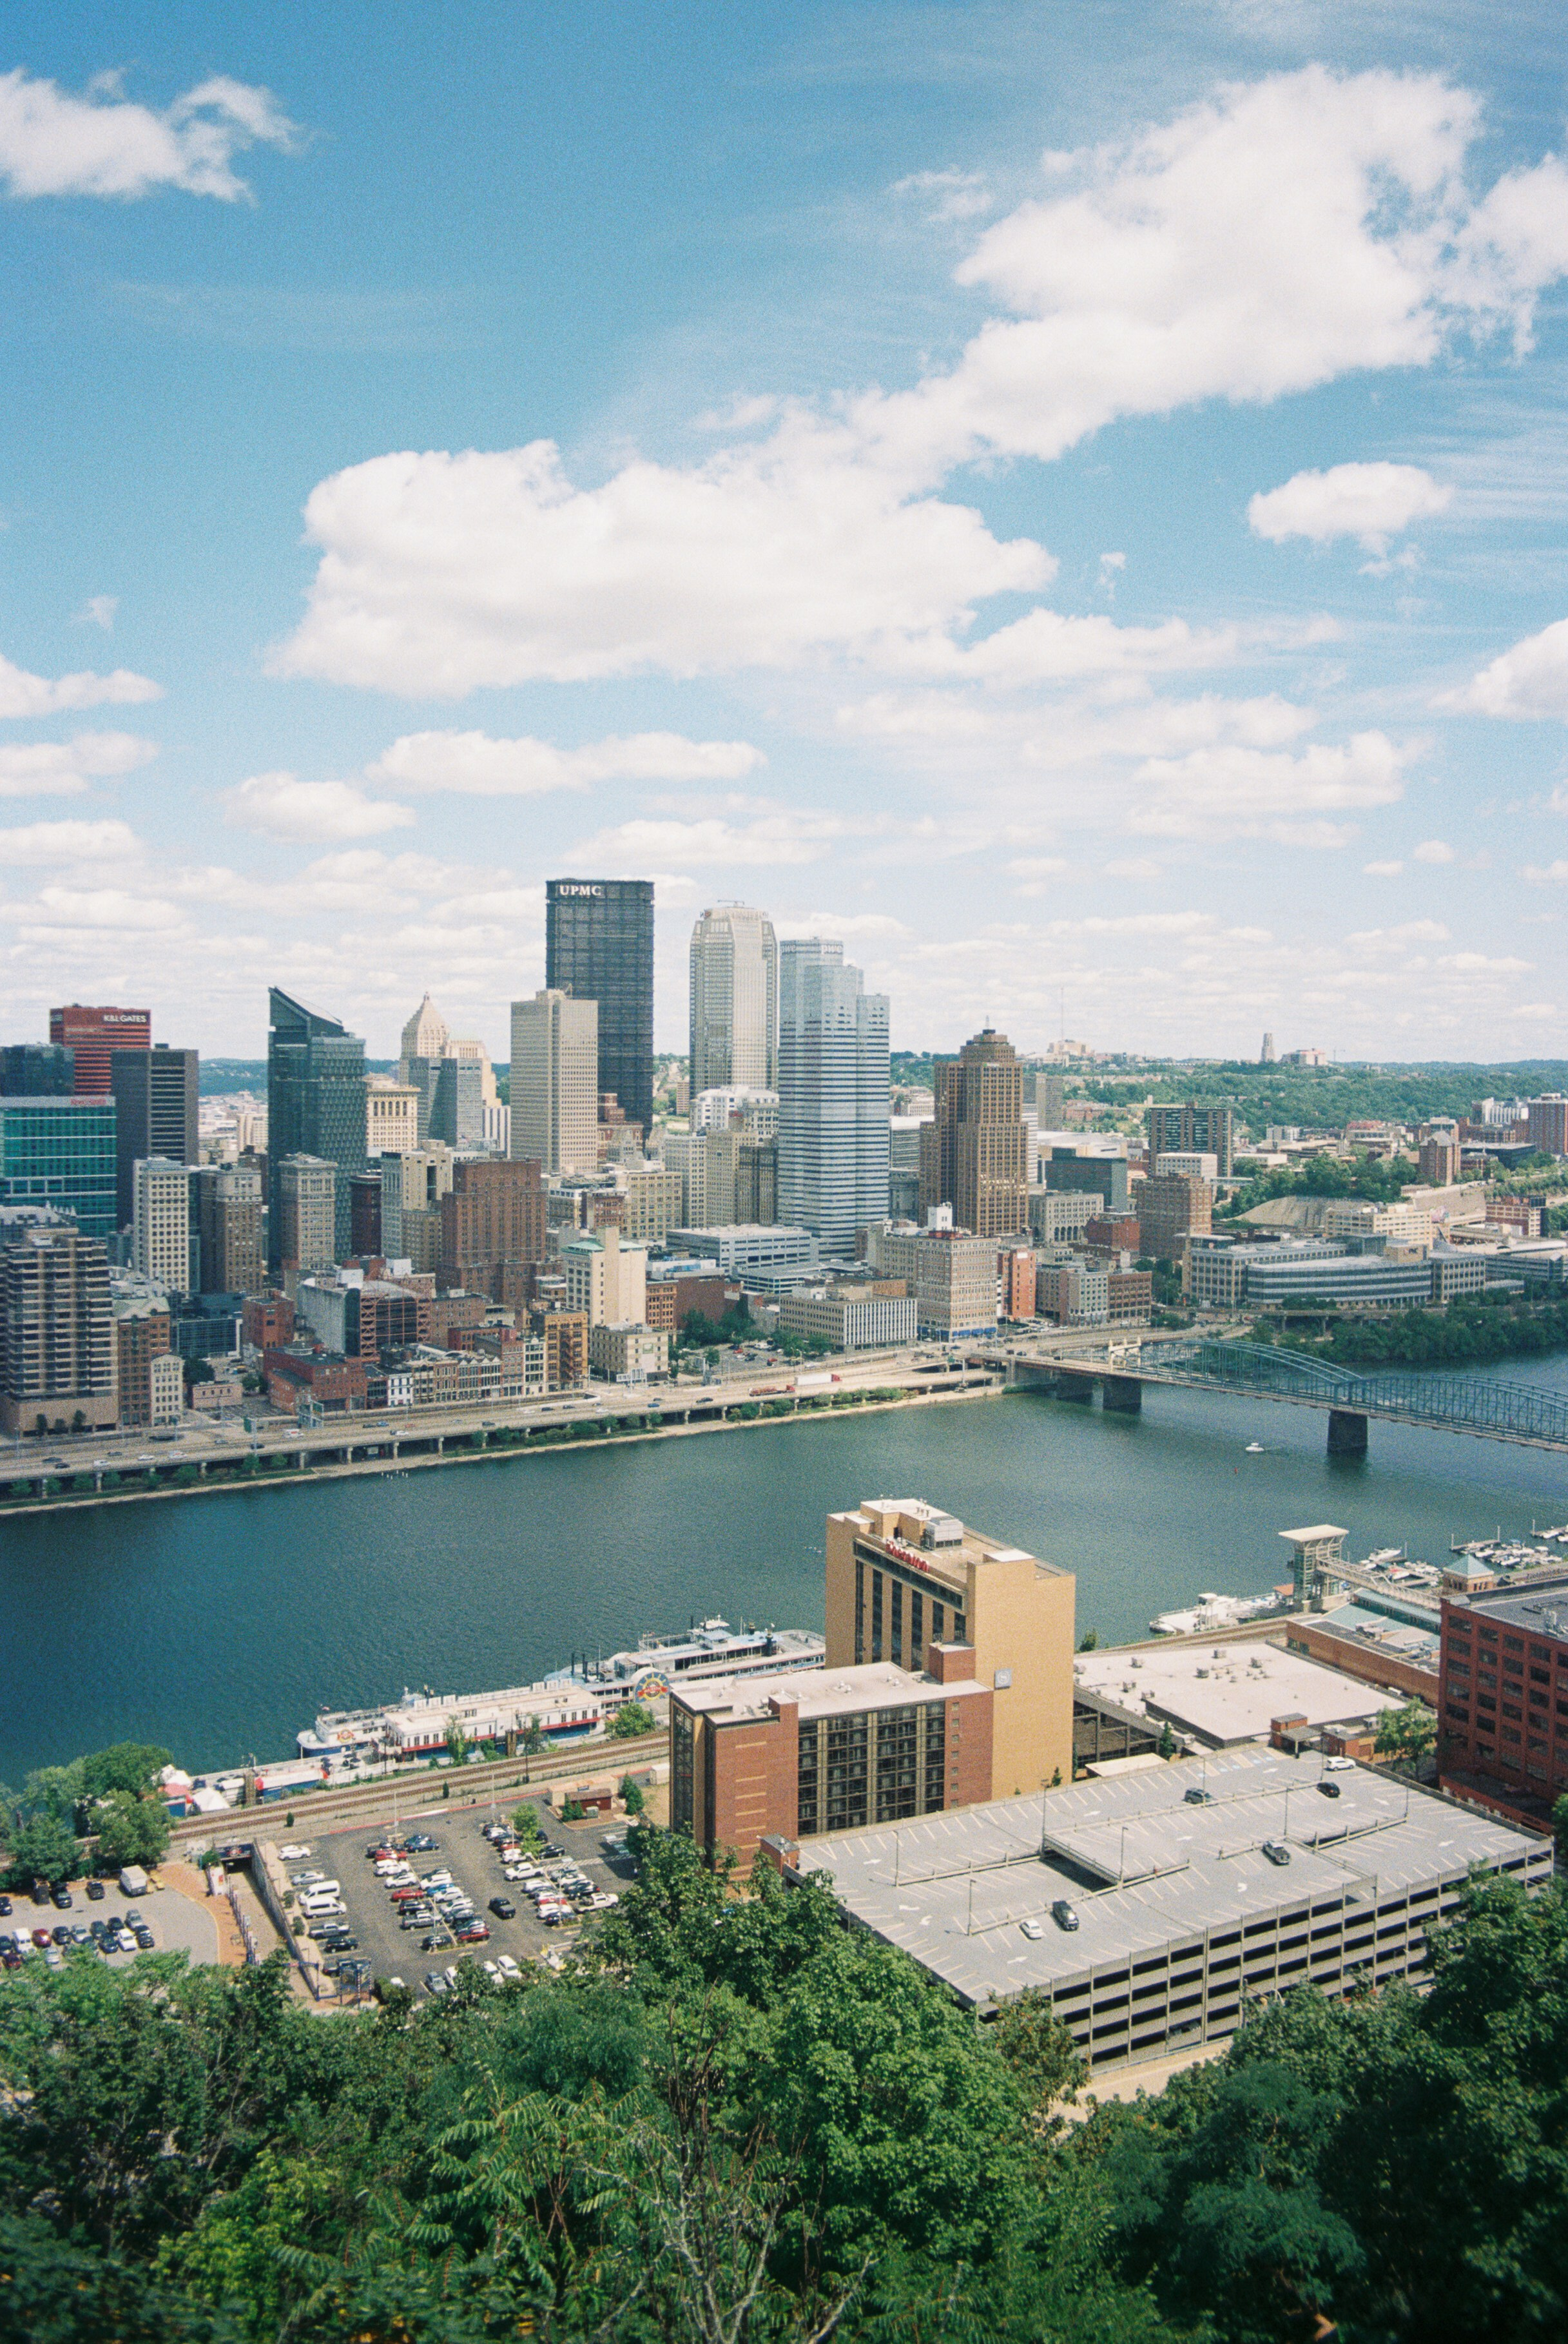
\includegraphics[scale=0.385]{./Images/banner.jpg}}} % Image background
\centering
\vspace*{5cm}
\par\normalfont\fontsize{35}{35}\sffamily\selectfont
\textbf{CHE374H1 Fall 2024}\\
{\LARGE Engineering Economic Analysis and Decision Making}\par % Book title
\vspace*{1cm}
{\Huge Nasrudeen Oladimeji}\par % Author name
\endgroup

%----------------------------------------------------------------------------------------
%	COPYRIGHT PAGE
%----------------------------------------------------------------------------------------

\newpage
~\vfill
\thispagestyle{empty}

%\noindent Copyright \copyright\ 2014 Andrea Hidalgo\\ % Copyright notice

\noindent\textsc{University of Toronto}\\

\noindent \textsc{github.com/Nasr-905}\\ % URL

\noindent Professor: Yuri Lawryshyn (yuri.lawryshyn@utoronto.ca)\\ % License information

\noindent \textit{First release, September 2024} % Printing/edition date

%----------------------------------------------------------------------------------------
%	TABLE OF CONTENTS
%----------------------------------------------------------------------------------------

\chapterimage{./Images/head1.jpg} % Table of contents heading image

\pagestyle{empty} % No headers

\tableofcontents % Print the table of contents itself

%\cleardoublepage % Forces the first chapter to start on an odd page so it's on the right

\pagestyle{fancy} % Print headers again

% theorem
% problem
% example
% vocabulary
% definition
% corollary - statement that follows immediately from a theorem/proof.
% remark
% proof
% lemma - An intermediate theorem used to prove something larger
% observation - A noteworthy or interesting point
% proposition - A statement that is not as important as a theorem
% claim -  A statement presented as true, to be proven within the text.
% fact A statement known to be true, used without needing a detailed proof
% assumption - A statement that is taken to be true without proof

\chapterimage{./Images/head2.jpg} % Chapter heading image
\chapter{The Introduction}


\chapter{Cash-flow Analysis}

\section{Cash-flows}
\begin{definition}
    [Cash-flow]
    A \textit{cash-flow} is a series of cash receipts and payments, they can be positive or negative.
\end{definition}
\begin{itemize}
    \item First (Capital) Cost - the initial cost of an investment
    \item Revenues (Sales) - cash inflows from the sale of goods or services
    \item Operations and Maintenance (O\&M) - cash outflows for the operation and maintenance of the investment
    \item Overhaul and Replacement - cash outflows for the overhaul and replacement of the investment
    \item Salvage Value - cash inflows from the sale of the investment at the end of its useful life
    \item Scrap Value - cash inflows from the sale of the investment at the end of its useful life
    \item Disposal Cost - cash outflows for the disposal of the investment at the end of its useful life
\end{itemize}

\begin{definition}
    [Project Life-cycle Cost]
    Costs that occur at the start, during, or end of a project.
\end{definition}

\begin{figure}[H]
    \centering
    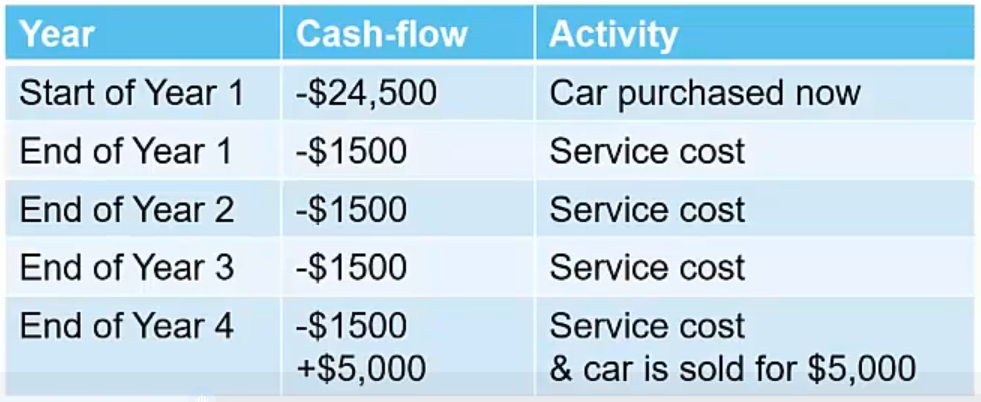
\includegraphics[width=0.8\textwidth]{LECTURE_2/cash-flow_table.png}
    \caption{Cash-flow Table}
    \label{fig:cash-flow_table}
\end{figure}

\begin{definition}
    [Cash-flow Diagram]
    A diagram that shows the cash-flows of a project over time.
    \begin{itemize}
        \item X-axis: time, Y-axis: cash-flow
        \item Y-axis: size and direction of cash-flow
        \item Individual cash-flows are shown as arrows
              \begin{itemize}
                  \item Upward arrows: cash inflows (disbursements)
                  \item Downward arrows: cash outflows (recipts)
              \end{itemize}
        \item Time 0 is the beginning of period 1
        \item Cash-flows occuring during a period is assumed to have occured at the end of that period
        \item Interest is compounded at the end of each period
    \end{itemize}
\end{definition}
\begin{figure}[H]
    \centering
    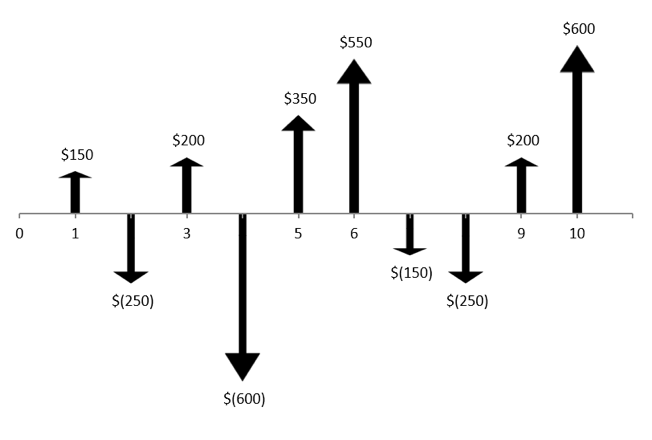
\includegraphics[width=0.8\textwidth]{LECTURE_2/cash-flow-diagram.png}
    \caption{Cash-flow Diagram}
    \label{fig:cash-flow_diagram}
\end{figure}

\begin{remark}
    Cash-flow diagrams from the lender's perspective is reversed from the borrower's perspective.
    % two side-by side diagrams
    \begin{figure}[H]
        \centering
        \begin{subfigure}[b]{0.4\textwidth}
            \centering
            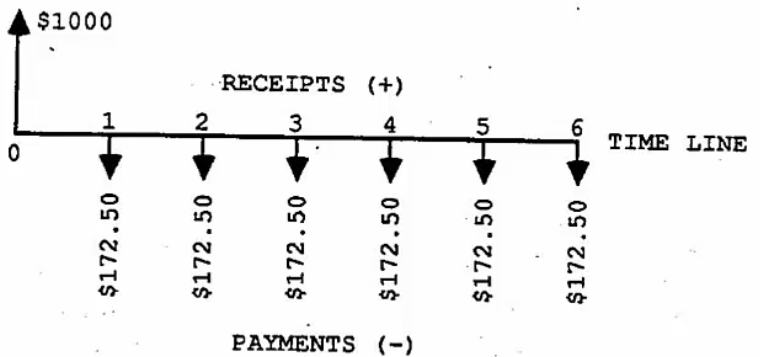
\includegraphics[width=\textwidth]{LECTURE_2/borrower_s_cash-flow.png}
            \caption{Borrower's Perspective}
            \label{fig:cash-flow_diagram_borrower}
        \end{subfigure}
        \begin{subfigure}[b]{0.4\textwidth}
            \centering
            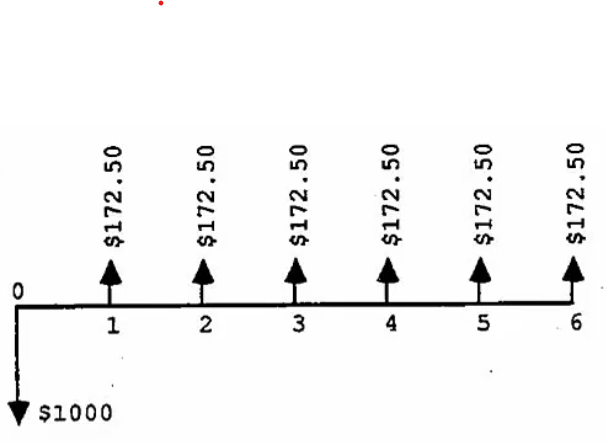
\includegraphics[width=\textwidth]{LECTURE_2/lender_s_cash-flow.png}
            \caption{Lender's Perspective}
            \label{fig:cash-flow_diagram_lender}
        \end{subfigure}
        \caption{Cash-flow Diagrams}
        \label{fig:cash-flow_diagrams}
    \end{figure}
\end{remark}

\begin{example}
    Young Professional: Çonstruct a cash-flow diagram with the
    following cash-flows (assume 4 weeks per month)
    $\cdot$ Monthly income:  \$ 2200( received at the end of each' month)
    Rent includes utilities: \$700 (at the end of each month)
    Weekly food and entertainment: \$120
    Telephone bill: \$40 (at the end of the first week of each month)
    Credit card purchases: \$300 (at the end of the second week of each
    month)
    \begin{figure}[H]
        \centering
        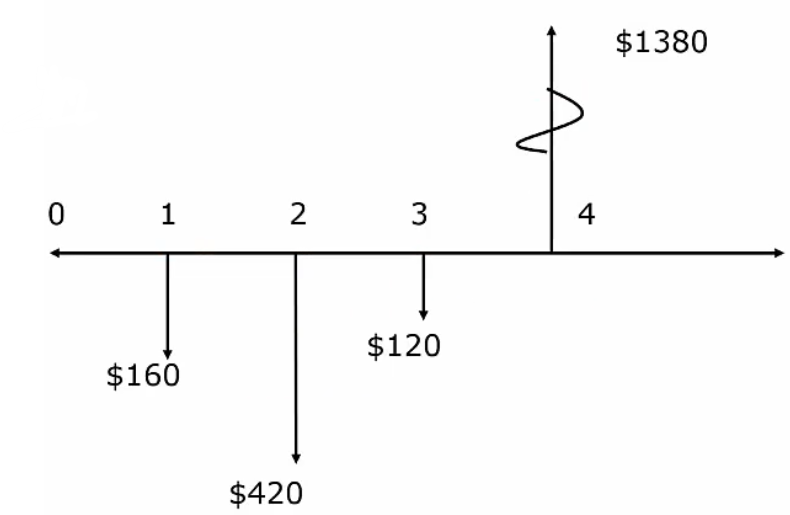
\includegraphics[width=0.8\textwidth]{LECTURE_2/cash-flow-ex.png}
        \caption{Young Professional Cash-flow Diagram}
        \label{fig:young_professional_cash-flow}
    \end{figure}
\end{example}

\section{Cash-flow Categories}

\begin{definition}
    [Single Payments/ Receipts]
    Cash-flows that occur only once.
\end{definition}

\begin{definition}
    [Perpetuity]
    Cash-flows that occur indefinitely.
\end{definition}
\begin{figure}[H]
    \centering
    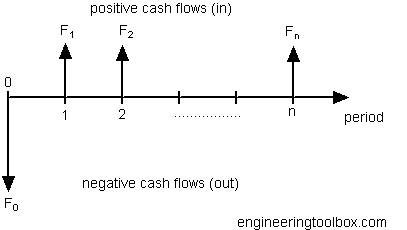
\includegraphics[width=0.8\textwidth]{LECTURE_2/perpetuity.png}
    \caption{Perpetuity Cash-flow Diagram ($n \to \infty$)}

\end{figure}

\begin{definition}
    [Annuity]
    Cash-flows that occur at regular intervals (e.g. coupon payments, bonds, etc.)
\end{definition}
\begin{figure}[H]
    \centering
    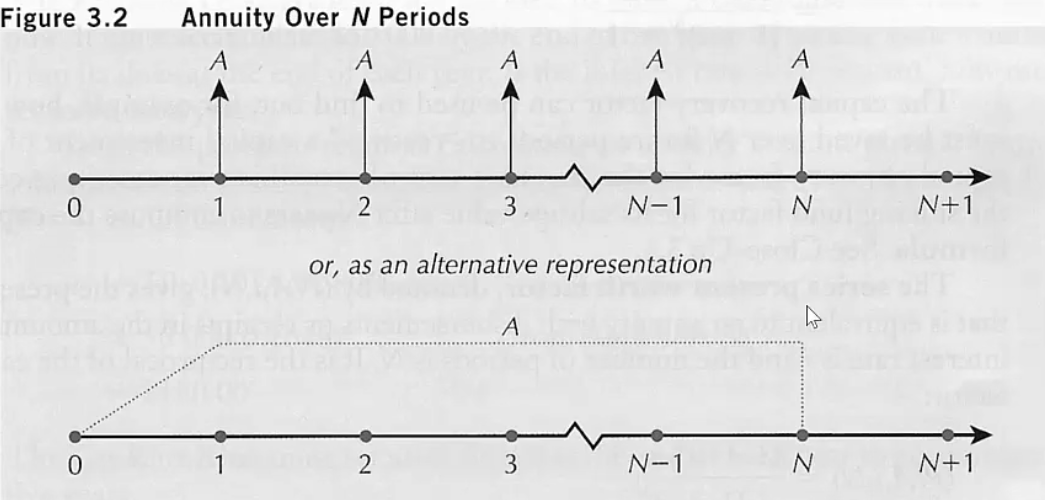
\includegraphics[width=0.8\textwidth]{LECTURE_2/annuity.png}
    \caption{Annuity Cash-flow Diagram}
    \label{fig:annuity_cash-flow}
\end{figure}

\begin{definition}
    [Arithmetic Gradient]
    Cash-flows that increase or decrease by a constant amount at regular intervals.
    \begin{equation}
        A_n = A' + (N-1)G
    \end{equation}
    Where:
    \begin{itemize}
        \item $A'$ is the original amount
        \item $G$ is the amount added
        \item $N$ is the number of periods
    \end{itemize}
\end{definition}
\begin{figure}[H]
    \centering
    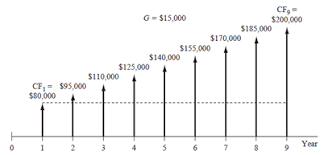
\includegraphics[width=0.8\textwidth]{LECTURE_2/arithmetic_gradient.png}
    \caption{Arithmetic Gradient Cash-flow Diagram}
    \label{fig:arithmetic_gradient_cash-flow}
\end{figure}

\begin{definition}
    [Geometric Gradient]
    Cash-flow that grows exponentially such that if $A$ is the principal cash-flow, then the cash-flow at period $N$ is $A_N = A(1+g)^{N-1}$
\end{definition}

\begin{figure}[H]
    \centering
    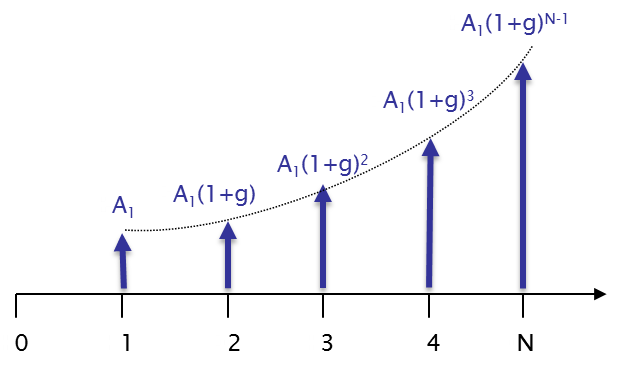
\includegraphics{LECTURE_2/geometric-gradient-series.png}
    \caption{Geometric Cash-flow Diagram}
    \label{geom-cash-flow}
\end{figure}

\section{Cash-flow Equivalence}

\subsection{Mathematical Equivalence}
\begin{definition}
    [Mathematical Equivalence]
    Two cash-flows, $P_t$ at time $t$ and $F_{t+N}$ at time $t+N$ are mathematically equivalent if, at a certain interest rate $i$, they have the same present value or future value:
    \[
        F_{t+N} = P_t(1+i)^N
    \]
    \textit{If the time changes, the magnitude of the cash-flow changes accordingly.}
\end{definition}

\begin{figure}[H]
    \centering
    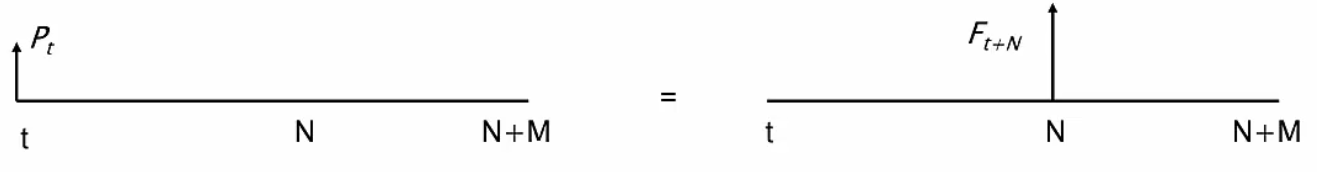
\includegraphics[width=0.8\textwidth]{LECTURE_2/mat-equiv.png}
    \caption{Mathematical Cash-flow Diagram}
    \label{fig:mathematical_cash-flow}
\end{figure}

\begin{definition}
    [Market Equivalence]
    The ability to exchange cash-flows in the market without any loss. \\
    \begin{itemize}
        \item Exchanging $P_t$ for $F_{t+N}$ at time $t$ is lending money.
        \item Exchanging $F_{t+N}$ for $P_t$ at time $t$ is borrowing money.
    \end{itemize}
\end{definition}

\begin{example}
    [Treasury Bills]
    A Treasury Bill(T-bill) is a short-term government debt obligation backed by the government with a maturity of one year or less. T-bills are usually sold in denominations of $\$1,000$. If a $\$1000$ T-bill due to mature in 6 months is currently selling for $\$990.10$ then that means some investors holding the Tbill are willing to sell them at this price while others are willing to buy them at this price. The“market” has agreed that the appropriate interest rate is 1\% over 6 months. Confirm this by calculating the yield.
    \begin{align*}
        FV   & = \$1000                      \\
        PV   & = \$990.10                    \\
        N    & = 0.5 \text{ years}           \\
        i    & = ?                           \\
        FV   & = PV(1+i)^N                   \\
        1000 & = 990.10(1+i)^{0.5}           \\
        1+i  & = {\frac{1000}{990.10}}^2     \\
        i    & = {\frac{1000}{990.10}}^2 - 1 \\
        i    & \approx 0.01
    \end{align*}
\end{example}

\begin{definition}
    [Decisional Equivalence]
    The indifference of an investor to choose between two cash-flows, e.g. $P_t$ at time $t$ and $F_{t+N}$ at time $t+N$.
\end{definition}

\begin{example}
    \begin{itemize}
        \item Need: 1,000 kg aluminium on August 15
        \item Offer: 1,100 kg aluminium on August 22
        \item Same price and payment at the end of August
        \item An implied interest rate offer of 10\% for a week
    \end{itemize}
    The question is: How much is it worth for decision maker to accept the delay in delivery? \\
    If the manufacturer has a lot of aluminum in stock, it may be worth it to wait a week to get the extra 100 kg. If the manufacturer is running low on aluminum, the manufacturer may have to pay in penalties, or pay workers over-time to meet the deadline.
\end{example}



\section{Cash-flow Factors}

\begin{theorem}
    [Factor Notation]
    \begin{itemize}
        \item $(X/Y, i, N)$ - the factor that converts one kind of cash-flow to another
              \begin{itemize}
                  \item $X$ and $Y$ are one of the following:
                        \begin{itemize}
                            \item $F$ - future value
                            \item $P$ - present value
                            \item $A$ - annual value
                            \item $G$ - gradient
                            \item $g$ - growth rate
                        \end{itemize}
                  \item So, to convert from a present value $P$ to a future value $F$ at interest rate $i$ for $N$ periods, we use the factor $(P/F, i, N)$, which is read as "P given F at i for $N$ periods"
                  \item For the geometric gradient, we use $P = (P/G, i, g, N)$
              \end{itemize}
        \item Some factors have specific names
              \begin{itemize}
                  \item $(F/P, i, N)$ - Compound amount factor
                  \item $(P/F, i, N)$ - Present worth factor
                  \item $(A/F, i, N)$ - Sinking fund factor
                  \item $(F/A, i, N)$ - Series compound amount factor
                  \item $(A/P, i, N)$ - Capital recovery factor
                  \item $(P/A, i, N)$ - Series present worth factor
              \end{itemize}
    \end{itemize}
\end{theorem}

\begin{corollary}
    [Compound Amount Factor]
    \[
        F = P(1+i)^N
    \]
    \[
        (F/P, i, N) = (1+i)^N
    \]
\end{corollary}

\begin{example}
    If you had \$2000 now and invested it at 10\% interest, how much would you have in 8 years? \\
    \textbf{Solution:}
    \begin{align}
        P & = 2000, i = 0.1, N = 8 \\
        F & = P(P/F, i, N)         \\
        F & = 2000(P/F, 10\%, 8)   \\
        F & = 2000(1+0.1)^8        \\
        F & = 2000(2.143)          \\
        F & = 4287.20
    \end{align}
\end{example}
\begin{definition}
    [Present Worth Factor]
    \begin{align}
        P           & = \frac{F}{(1+i)^N} \\
        (P/F, i, N) & = \frac{1}{(1+i)^N} \\
        (F/P, i, N) & = (1+i)^N
    \end{align}
\end{definition}

\begin{definition}
    [Discount Rate]
    The interest rate used to convert future cash-flows to present value.\\
    For example, if you invest \%100 at 5\% interest, you expect to have $F = P \times (1+i) = \$100\times(1.05) = \$105$ at the end of the year. Therefore:
    \[
        P = \frac{F}{(1+i)^N} \qquad i \text{ is the discount rate, $N$ is the number of periods}
    \]
\end{definition}

\begin{corollary}
    [Discount Rate Using Continuous Compounding]
\begin{align}
    P & = \frac{F}{(1+i)^N} \\
    & = \frac{F}{(1 + e^r - 1)^N} \\
    & = \frac{F}{e^{rN}}
\end{align}
\end{corollary}

\begin{definition}
    [Present Value of a Perpetuity]
    \begin{align}
        P & = \frac{A}{1 + i} + \frac{A}{(1+i)^2} + \frac{A}{(1+i)^3} + \ldots = \frac{A}{i}
    \end{align}
\end{definition}

\begin{definition}
    [Present Value of an Annuity]
    The present value of an annuity is equal to a perpetuity starting at the first period minus a perpetuity of the same size starting at the $N+1$ period.
    \begin{align}
        P          & = A(P/A, i, N) = P_1 - P_2                                  \\
        P_1        & = \frac{A}{i}                                               \\
        P_2        & = \frac{A}{i}(1+i)^{-N}                                     \\
        P          & = A(\frac{1}{i} - \frac{1}{i}(1+i)^{-N})                    \\
        \therefore & \boxed{(P/A, i, N) = \frac{1}{i}( 1 - \frac{1}{(1+i)^{N}})}
    \end{align}
    \textit{Note: The second annuity, like all annuities, is also worth $A/i$, but because it starts at the $N+1$ period, we discount it.}
\end{definition}


\begin{definition}
    [Present Value of an Arithmetic Growth Factor]
    The arithmetic gradient is the sum of $N$ annuities, each increasing by a constant amount $G$. Remember that arithmetic gradients begin at period 1.
    \begin{align*}
        P           & = G(P/G, i, N) =                                                                                                                                                           \\
        P           & = G \left(\frac{(P/A, i, n-1)}{1 + i} + \frac{(P/A, i, n-2)}{(1 + i)^2} + \cdots + \frac{(P/A, i, 1)}{(1+i)^{n-1}}\right)                                                  \\
        \rightarrow & \quad \text{remember that } (P/A, i, N) = \frac{1}{i}\left(1 - \frac{1}{(1+i)^a}\right)                                                                                    \\
        P           & = \frac{G}{i} \left(
        \frac{1}{1+i} + \frac{1}{(1+i)^2} + \cdots + \frac{1}{(1+i)^{N-1}}
        \right)                                                                                                                                                                                  \\
                    & + \frac{G}{i} \left(
        - \frac{1}{(1+i)}\frac{1}{(1+i)^{N-1}} - \frac{1}{(1+i)^2}\frac{1}{(1+i)^{N-2}} - \cdots - \frac{1}{(1+i)^{N-1}}\frac{1}{1}
        \right)                                                                                                                                                                                  \\
        \rightarrow & \text{ The first term resembles an annuity, so we can add $\frac{1}{(1 + i)^N}$ to complete it}                                                                            \\
        P           & = \frac{G}{i}\left(                                    \frac{1}{1+i} + \frac{1}{(1+i)^2} + \cdots + \frac{1}{(1+i )^N} - \frac{1}{(1+i)^N} - \frac{n -1}{(1 + i)^N}\right)
        \\
        P           & = \frac{G}{i}\left(\frac{1}{i}(1 - \frac{1}{(1 + i)^N}) - \frac{N}{(1 + i)^N}\right)                                                                                       \\
        P           & = \frac{G}{i^2}\left(1 - \frac{1+iN}{(1 + i)^N}\right)                                                                                                                     \\
        \therefore  & \boxed{(P/G, i, N) = \frac{1}{i^2}\left(1 - \frac{1+iN}{(1 + i)^N}\right)}
    \end{align*}
    \textit{Note: To get the total arithmetic gradient present value, add the growth factor to the initial annuity such that: $P = A(P/A, i, N) + G(P/G, i, N)$}
\end{definition}

\begin{definition}
    [Present Value of a Geometric Gradient]
    Looking at the figure \ref{geom-cash-flow}, we can model the present value of a geometric gradient, keeping in mind to discount the cash-flows at the end of each period.
    \begin{align*}
        P           & = \frac{A}{1 + i} + \frac{A(1+g)}{(1+i)^2} + \ldots + \frac{A(1+g)^{N-1}}{(1+i)^N}                                   \\
        P           & = \frac{A}{1 + g}\left(
        \frac{1 + g}{1 + i} + \frac{(1 + g)^2}{(1 + i)^2} + \ldots + \frac{(1 + g)^{N}}{(1 + i)^{N}}
        \right)                                                                                                                            \\
        \rightarrow & \text{ Let's define } \frac{1}{1 + i^0} = \frac{1+g}{1+i} \iff i^0 = \frac{1 + i}{1 + g} -1                          \\
        P           & = \frac{A}{1 + g} ( \frac{1}{1 + i^0} + \frac{1}{(1 + i)^2} + \ldots + \frac{1}{(1 + i)^N})                          \\
        \rightarrow & \text{ We can use the present value of an annuity to simplify this}                                                  \\
        P           & = \frac{A}{1 + g} (P/A, i^0, N)                                                                                      \\
        P           & = A \times \frac{1 - (\frac{1 + g}{1 + i})^N}{i - g}                                                                 \\
        \therefore  & \boxed{(P/G, i, g, N) =\begin{aligned}
                                                                & \frac{1 - (\frac{1 + g}{1 + i})^N}{i - g}                                     \\
                                                     \text{or } & \frac{(P/A, i^0, N)}{1 + g} \quad \text{where } i^0 = \frac{1 + i}{1 + g} - 1
                                                 \end{aligned}}
    \end{align*}
\end{definition}

\section{Examples Using Cash-flow Factors}
\begin{example}
    [The Magic of Compound Interest]
    If you are 20 years old and save and invest \$1.00 each day, assume you live to age 80 and the annual interest rate is 10\%, you can become a millionaire! Let's verify
    \textbf{Solution:}
    First convert annual interest to daily interest:
    \begin{align}
        (1 + r)^365&  = 1 + 0.1 \\
        r          & = 0.02612\% \\
        F = \$ 1 \times (A/F, 0.02612\%, 60 \times 365) \\
        & = \$ 1 \times (F/P, 0.02612\%, 60 \times 365)\times (A/F, 0.02612\%, 60 \times 365) \\
        & = \$ 1.162 M\\
    \end{align}
\end{example} 

\begin{theorem}
    [Compounded Interest Rates]
    A yearly interest rate $r$ compounded $m$ times per year is equivalent to an interest rate $i_s = \frac{r}{m}$ per subperiod, such that:
    \begin{align}
        F & = P(1 + \frac{r}{m})^{mN} \\
        F & = P(F/P, \frac{r}{m}, mN)
    \end{align}
\end{theorem}


% \chapter{Financial Instruments: Mortgages and Bonds}

\section{Mortgages}

\begin{definition}
    A \textbf{mortgage} is a loan secured by the collateral of real estate property. The borrower is obligated to pay back the loan in a specified period of time. If the borrower fails to make the payments, the lender can take possession of the property.
\end{definition}

\begin{definition}
    [Principle]
    The \textbf{principle} is the amount of money borrowed from the lender. In the case of a mortgage, the principle is the percent of the house's value that the borrower did not pay upfront.
\end{definition}

\begin{definition}
    [Down Payment]
    The \textbf{down payment} is the amount of money paid upfront by the borrower. The down payment is a percentage of the house's value.
\end{definition}

\begin{definition}
    [Loan to Value Ratio]
    The \textbf{loan to value ratio} is the ratio of the principle to the value of the house. The loan to value ratio is calculated as follows:
    \[
        \text{LTV} = \frac{\text{Principle}}{\text{House Value}}
    \]
\end{definition}

\begin{definition}
    [Amortization Period]
    The \textbf{amortization period} is the amount of time it takes to pay off the mortgage. The amortization period is typically 25 years.
\end{definition}

\begin{definition}
    [Mortgage Rate]
    The \textbf{mortgage rate} is the interest rate on the mortgage. The mortgage rate is typically 2-3\%.\\
    \textit{Note: The mortgage rate is given as an \textbf{annual rate}.}
\end{definition}

\begin{definition}
    [Mortgage Term]
    The \textbf{mortgage term} is the amount of time the mortgage rate is fixed. After which the mortgage rate is renegotiated.
    \\ The mortgage term is typically 5 years.
\end{definition}

\begin{example}
    [Mortgage Payment]
    Suppose you buy a house for \$500,000 with a 20\% down payment. You take out a mortgage with a 5\% interest rate, a 5 year term, and a 25 year amortization period. \\
    a) What is your monthly payment during this term?
    \begin{align*}
        P_1 &= 400,000 \quad &\text{(Principle)}\\
        i_1 &= 0.05 \quad &\text{(Mortgage Rate)}\\
        N_1 &= 25\times 12 = 300 \quad &\text{(Number of Payments)}\\
        A_1 &= P \cdot (A/P, i_1, N_2)\\
        &= \$ 2338
    \end{align*}    
    b) After the end of the term, the new mortgage rate is 6\%. What is your new monthly payment?
    \begin{align*}
        i_2 &= 0.06 \quad &\text{(New Mortgage Rate)}\\
        P_2 &= P_1\cdot (F/P, i_1, 5\times 12) &\text{(Principle after 5 years)}\\
        & - A_1\cdot (F/A, i_2, 5\times 12) &\text{(Payments after 5 years)}\\
        & = \$354,320 \\
        N_2 &= 20\times 12 = 240 \quad &\text{(Number of Payments)}\\
        A_2 &= P_2\cdot (A/P, i_2, N)\\
        &= \$ 2,538
    \end{align*}
\end{example}

\section{Bonds}

\begin{definition}
    [Bond]
    A \textbf{bond} is a fixed income instrument that represents a loan made by an investor to a borrower. The borrower is typically a corporation or government. The borrower agrees to pay the investor a fixed interest rate over a specified period of time (usually 10-30 years).
\end{definition}

\begin{definition}
    [Face Value]
    The \textbf{face value} is the amount of money the bondholder will receive at the end of the bond's term. The face value is also known as the \textbf{par value}.
\end{definition}

\begin{figure}[H]
    \centering
    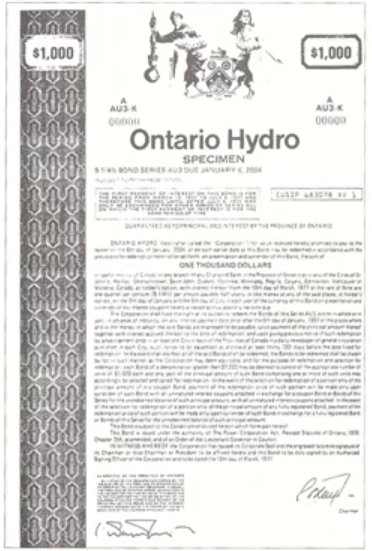
\includegraphics[width=0.5\textwidth]{LECTURE_3/bond-face.png}
    \caption{Bond Front/Face}
\end{figure}

\begin{definition}
    [Coupon Rate]
    The \textbf{coupon rate} is the interest rate that the bondholder will receive annually as a percentage of the face value. The coupon rate is typically 2-3\%.
\end{definition}

\begin{theorem}
    [Cash Flow Comparison]
    It is common that cash flows are compared to the current interest rate you would receive if you invested the same amount of money in a savings account. This is because the banks are considered to be the safest investment.
\end{theorem}

\subsection{Risk and Reward}
\begin{definition}
    [Yield Rate]
    The \textbf{yield rate} is the rate of return on an investment. The yield rate is the interest rate that makes the present value of the investment's cash flows equal to the bond's price. \\
    On the flip side, the yield rate is the amount you (or the market) is willing to pay for the investment due to it's perceived risk.
\end{definition}
\begin{example}
    [Bond Cash Flow Comparison]
    Suppose you buy a bond with a face value of \$1000, a coupon rate of 5\%, and a term of 10 years.\\
    The bank is paying 10\% interest. What is the equivalent amount you would need to put into the bank now in order to get the same cash flows?
    \begin{align*}
        i_{\text{Bank}} &= 0.1/2 = 0.05 \quad &\text{(Bank Rate Semi-annually)}\\
        i_{\text{Bond}} &= 0.05 \quad &\text{(Bond Rate)}\\
        N &= 10\times 2 = 20 \quad &\text{(Number of Payments)}\\
        A &= 1000\times i_{\text{Bond}} =\$ 46.25 &\text{(Semi-annual Payment)}\\
        F &= 1000 &\text{(Face Value)}\\
        P &= F\cdot (P/F, i_{\text{Bank}}, N) + A\cdot (P/A, i_{\text{Bank}}, N)\\
        & = \$ 953
    \end{align*}
    So, you would need to put \$953 in the bank to get the same cash flows as the bond. Do you trust the bond issuer as much as the bank? \\
    \textbf{Say that we don't trust the bond issuer as much as the bank.} \\
    Let's say the market is only willing to pay \$ 700 for the bond. What is the yield rate?
    \begin{align*}
        P &= 700 \quad &\text{(Bond Price)}\\
        i_{\text{yield}} &= ?\\
        P &= F\cdot (P/F, i_{\text{yield}}, N) + A\cdot (P/A, i_{\text{yield}}, N)\\
        i_{\text{yield}} &= 0.15\%
    \end{align*}
\end{example}

\section{Bonds Examples}


\begin{example}
    [Bond Price]
    A \$ 10,000 bond was bought that will mature in 8 years, it has a 12\% coupon payable quarterly. If the yield is 10\%, how much would you pay for the bond if it was for sale? \\
    \textbf{First we calculate the coupon payment:}
    \begin{align*}
        i &= 0.12/4 = 0.03 \quad &\text{(Coupon Rate)}\\
        A &= 10,000 \times 0.03 = \$ 300 &\text{(Quarterly Payment)}
    \end{align*}
    \textbf{Then we calculate the bond price:}
    \begin{align*}
        i_{\text{yield}} &= 0.1/4 = 0.025 \quad &\text{(Yield Rate)}\\
        N &= 8\times 4 = 32 \quad &\text{(Number of Payments)}\\
        P &= 300\cdot (P/A, 0.025, 32) + 10,000\cdot (P/F, 0.025, 32)\\
        &= \$ 11,092
    \end{align*}
\end{example}



% \chapter{Risk, Reward and Arbitrage}


\section{Capital Asset Pricing Model (CAPM)}

\subsection{Valuation}

\begin{definition}
    Valuation is the analytical process of determining the current (or projected) worth of an asset or a company. \\
    \textbf{Components of a valuation:}
    \begin{itemize}
        \item \textbf{Projected cash flows:} The expected future cash flows of the asset or company.
        \item \textbf{Interest/hurdle rate:} The rate of return required by the investor to invest in the asset or company.
    \end{itemize}
\end{definition}

\begin{definition}
    [Pricing Risk]
    Pricing risk is the process of determining the appropriate interest rate (rate of return) for an asset or company based on the risk associated with the asset or company.
\end{definition}

\begin{theorem}
    [Project/Company Returns]
    Say you have a portfolio of $n$ stocks, and the price of the $i^{th}$ stock is given in table \ref{tab:time_period_price}. The returns of a project/company (stock) at time $t_j$ is given by:
    \begin{equation}
        P_{t_j} = P_{t_{j-1}} e^{r_{t_{j}}\Delta t}
    \end{equation}
    Because we are dealing with continuous compounding.\\
    We can find the rate of return $r_{t_{j}}$ by:
    \begin{equation}
        r_{t_{j}} = \frac{1}{\Delta t} \ln\left(\frac{P_{t_j}}{P_{t_{j-1}}}\right)
    \end{equation}
    The return vector for the $i^{th}$ stock is given by:
    \begin{equation}
        \overrightarrow{R_i} =  \begin{bmatrix}
            r_{t_1} \\
            r_{t_2} \\
            \vdots  \\
            r_{t_n}
        \end{bmatrix}
    \end{equation}
\end{theorem}

\begin{table}[h!]
    \centering
    \begin{tabular}{|c|c|}
        \hline
        \textbf{Time Period (t)} & \textbf{Price (P)} \\ \hline
        0                        & 20                 \\ \hline
        1                        & 21                 \\ \hline
        2                        & 22                 \\ \hline
        3                        & 20                 \\ \hline
        4                        & 21                 \\ \hline
    \end{tabular}
    \caption{Time Period vs. Price}
    \label{tab:time_period_price}
\end{table}

\begin{definition}
    [Volatility]
    Volatility is a statistical measure of the dispersion of returns for a given security or market index.
    Volatility is the standard deviation of the returns.
    \begin{equation}
        \sigma = \sqrt{Var(\overrightarrow{R_i})} = \sqrt{\frac{1}{n-1} \sum_{i=1}^{n} (r_i - \bar{r})^2}
    \end{equation}
    where:
    \begin{itemize}
        \item $r_i$ is the return at time $i$.
        \item $\bar{r}$ is the average return.
        \item $n$ is the number of returns.
    \end{itemize}
\end{definition}

\begin{proposition}
    [Modern Portfolio Theory]
    \textbf{Objective:} To maximize the expected return, while minimizing volatility/risk ($\sigma$).\\
\end{proposition}
\begin{definition}
    [Covariance]
    The covariance between two assets is a measure of how the two assets move together. If the covariance is positive, the assets move together, i.e. when one asset increases, the other asset also increases.
    \begin{equation}
        Cov(\overrightarrow{R_i},\overrightarrow{R_j}) = \frac{1}{n-1} \sum_{i=1}^{n} (r_{i} - \bar{r_i})(r_{j} - \bar{r_j})
    \end{equation}
\end{definition}

\begin{lemma}
    [Purpose of Covariance]
    Having positive covariances across your assets should increase your volatility, because if one crashes, the others are likely to crash as well. So in general, we want negative, or at least low, covariances.\\
\end{lemma}

\begin{definition}
    Assume we can proportionally invest in $x_i$ amount in the $i^{th}$ asset. We define:
    \begin{equation}
        \overrightarrow{X} = \begin{bmatrix}
            x_1    \\
            x_2    \\
            \vdots \\
            x_n
        \end{bmatrix}
    \end{equation}
    And the covariance matrix of the returns of the $n$ assets is given by:
    \begin{equation}
        \Sigma = \begin{bmatrix}
            \sigma_{11} & \sigma_{12} & \cdots & \sigma_{1n} \\
            \sigma_{21} & \sigma_{22} & \cdots & \sigma_{2n} \\
            \vdots      & \vdots      & \ddots & \vdots      \\
            \sigma_{n1} & \sigma_{n2} & \cdots & \sigma_{nn}
        \end{bmatrix}
    \end{equation}
    Where:
    \begin{itemize}
        \item $\sigma_{ij} = \sigma_{ji} = Cov(\overrightarrow{R_i},\overrightarrow{R_j})  $ is the covariance between the $i^{th}$ and $j^{th}$ asset.
        \item $\sigma_{ii} = Var(\overrightarrow{R_i})$ is the variance of the $i^{th}$ asset.
    \end{itemize}
\end{definition}


\begin{definition}
    [Portfolio Expected Return]
    The expected return of a portfolio is given by:
    \begin{equation}
        \mathbb{E}[\overrightarrow{R_p}] = x_1 \mathbb{E}[\overrightarrow{R_1}] + x_2 \mathbb{E}[\overrightarrow{R_2}] + \cdots + x_n \mathbb{E}[\overrightarrow{R_n}] = \sum_{i=1}^{n} x_i \mathbb{E}[\overrightarrow{R_i}]
    \end{equation}
    Where:
    \begin{itemize}
        \item $\mathbb{E}[\overrightarrow{R_i}]$ is the expected return of the $i^{th}$ asset.
        \item $\mathbb{E}[\overrightarrow{R_p}]$ is the expected return of the portfolio.
        \item $\overrightarrow{R_i}$ is the historical return of the $i^{th}$ asset.
        \item $x_i$ is the proportion of the $i^{th}$ asset in the portfolio.
    \end{itemize}
    Intuitively, the expected return of each asset is multiplied by how much of the asset is in the portfolio.
\end{definition}

\begin{definition}
    [Portfolio Volatility]
    The volatility of a portfolio is given by:
    \begin{equation}
        \sigma_p = \sqrt{\overrightarrow{X}^T \times \Sigma \times \overrightarrow{X}}
    \end{equation}
\end{definition}

\begin{corollary}
    [Maximization]
    We want to maximize the expected return of the portfolio ($\mathbb{E}[\overrightarrow{R_p}]$) while minimizing the volatility of the portfolio ($\sigma_p$).\\
\end{corollary}

\begin{theorem}
    [CAPM Assumption]
    The Capital Asset Pricing Model (CAPM) assumes that investors are rational and risk-averse, in addition, it is just a model with numerous assumptions.\\
    \textbf{Assumptions:}
    \begin{itemize}
        \item Correlation and volatility of and between assets are fixed and constant forever
        \item All investors aim to maximize economic utility (i.e. make as much money as possible, regardless of any other considerations)
        \item[] \begin{itemize}
                  \item Although usually true, we see irrational behavior in the market (e.g. driven by fear)
              \end{itemize}
        \item All investors are rational and risk-averse
        \item All investors have access to the same information at the same time
        \item Investors have accurate conception of possible returns, i.e. the probability beliefs of investors match the true distribution of returns.
        \item There are no taxes or transaction costs
        \item[] \begin{itemize}
                  \item Often they are negligible, so they are ignored
              \end{itemize}
        \item All investors are price takers, i.e. their actions do not influence prices
        \item Any investor can lend and borrow an unlimited amount at the risk free rate of interest
        \item All securities can be divided into parcel of any size
    \end{itemize}
\end{theorem}

\begin{definition}
    [Efficiency Frontier]
    The efficiency frontier is the set of portfolios (expected returns and their respective volatilities, $\{(\mathbb{E}[R_p], \sigma_p)\}$) that satisfy the following conditions:
    \begin{align*}
        \text{Minimize:}   & \quad \sigma_p^2 = \overrightarrow{X}^T \Sigma \overrightarrow{X} \\
        \text{Subject to:} & \quad \sum_{i=1}^{n} x_i = 1                                      \\
                           & \quad \sum_{i=1}^{n} x_i \mathbb{E}[R_i] = \mathbb{E}[R_p]        \\
                           & \quad \sum_{i=1}^{n} x_i \sigma_i = \sigma_p
    \end{align*}
    Because $\sigma_p$ is squared, we can expect a parabolic shape for the curve. But the efficiency frontier is always the top half of the parabola, because we prefer a portfolio with a higher return for the same volatility.
\end{definition}
\begin{figure}[h!]
    \centering
    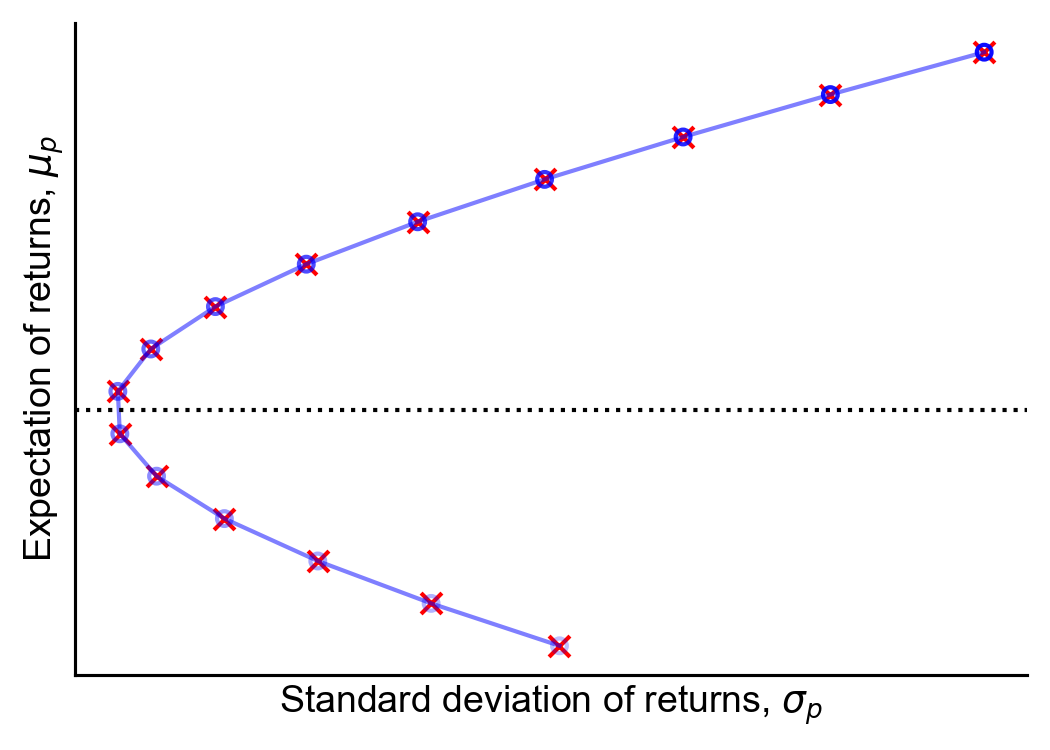
\includegraphics[width=0.6\textwidth]{LECTURE_4/efficient_frontier.png}
    \caption{Efficient Frontier}
    \label{fig:efficient_frontier}
\end{figure}

\begin{definition}
    [Tangency/Market Portfolio and Capital Market Line]
    Now we want to find the largest ratio of \textbf{excess} return to risk ($\frac{\mathbb{E}[R_p]}{\sigma_p}$).
    So we draw a tangent line that also intersects at the risk-free rate, $r_f$, this line is called the Capital Market Line (CML). The point where the tangent line intersects the efficient frontier is called the Tangency/Market Portfolio.\\
\end{definition}

\begin{definition}
    [Sharpe Ratio]
    To prove that this provides the largest ratio of excess return to risk, we realize that the slope of the tangent line is given by:
    \begin{align*}
        m & = \frac{y_2 - y_1}{x_2 - x_1}                \\
        m & = \frac{\mathbb{E}[R_p] - r_f}{\sigma_p - 0}
    \end{align*}
    This is the Sharpe Ratio, we want to maximize it, and it is the slope of the tangent line.\\
    Higher the slope, higher the sharpe ratio, higher the excess return for the same risk.
\end{definition}

\begin{figure}[h!]
    \centering
    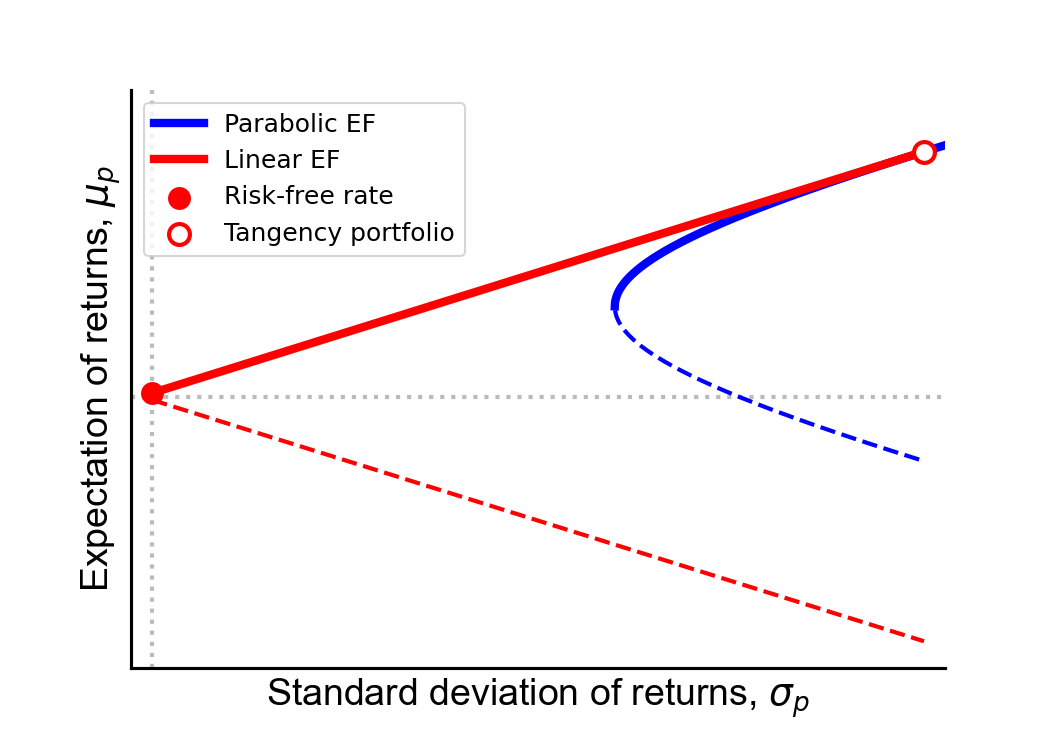
\includegraphics[width=0.6\textwidth]{LECTURE_4/CML.png}
    \caption{Capital Market Line}
    \label{fig:capital_market_line}

\end{figure}

\begin{proposition}
    [Leveraging Down/ Deleveraging]
    If we invest $50\%$ in the risk-free asset and $50\%$ in the market portfolio, we expect a return that is the average of the two returns, and a volatility that is the average of the two volatilities.\\
    \begin{equation}
        \mathbb{E}[R_{p}] = w\cdot \mathbb{E}[R_{m}] + (1-w)\cdot r_f
    \end{equation}

    \begin{equation}
        \sigma_{p} = \sqrt{w^2 \sigma_{m}^2 + (1-w)^2 \cdot \sigma_{f}}, \quad \sigma_{f} = 0
    \end{equation}
    Where $w$ is the weight of the market portfolio.\\
    This is called leveraging down, because we are investing in a less risky portfolio than the market portfolio.\\
\end{proposition}

\begin{lemma}
    Note that this can be done with any two points on the CML, not just the risk-free rate and the market portfolio.
\end{lemma}

\begin{proposition}
    [Leveraging Up]
    If we invest $150\%$ in the market portfolio and $-50\%$ (borrowing) in the risk-free asset, we expect a return that is $50\%$ higher than the market portfolio, and a volatility that is $50\%$ higher than the market portfolio.\\
    This is called leveraging up, because we are investing in a more risky portfolio than the market portfolio.\\
\end{proposition}


\begin{remark}
    It may seem weird at first that investing higher than the market portfolio suggests that we borrowed money at the risk-free rate. But this is just how the CAPM models riskier investments. This is because, in theory, no one would invest higher than the market portfolio, so the only way to achieve a higher return is to borrow money at the risk-free rate and invest more in the market portfolio.\\
\end{remark}

\begin{definition}
    [Stock Index]
    A stock index is a measure of the value of a section of the stock market. When the CAPM is applied to the stock market, the market portfolio is the stock index.\\
\end{definition}

\begin{definition}
    [Systematic Risk]
    Systematic risk is the risk that is inherent to the entire market or market segment. It is also known as undiversifiable risk or market risk $\beta$.\\
    E.g. If the economy is in a recession, all stocks will likely decrease in value.\\
\end{definition}

\begin{definition}
    [Idiosyncratic Risk]
    Idiosyncratic risk is the risk that is specific to a particular company or industry. It can be mitigated through diversification.\\
    E.g. If a company's CEO is caught embezzling money, the company's stock will likely decrease in value.\\
\end{definition}

\begin{proposition}
    You can 'portfolio' away idiosyncratic risk by diversifying your portfolio, but not systematic risk.\\
    \textbf{In the CAPM model, we assume everyone is logical and diversifies away idiosyncratic risk. So we only care about systematic risk.}
\end{proposition}

\begin{theorem}
    [Expected Return of an asset]
    The expected return of an asset is given by:
    \begin{equation}
        \mathbb{E}[R_i] = r_f + \beta_i(\mathbb{E}[R_m] - r_f)
    \end{equation}
    Intuitively, it says that the expected return of an asset is the risk-free rate plus the amount that an increase in the market portfolio would increase the return of the asset.\\
    The systematic risk of the asset is defined as:
    \begin{equation}
        \beta_i = \frac{Cov(R_i,R_m)}{Var(R_m)} = \frac{\sigma_{i,m}}{\sigma_{m}^2} = \frac{\rho_{i,m} \sigma_i}{\sigma_{m}}
    \end{equation}
    Plotting $\mathbb{E}[R_i]$ vs. $\beta_i$ gives the Security Market Line (SML).\\
\end{theorem}

\begin{figure}[h!]
    \centering
    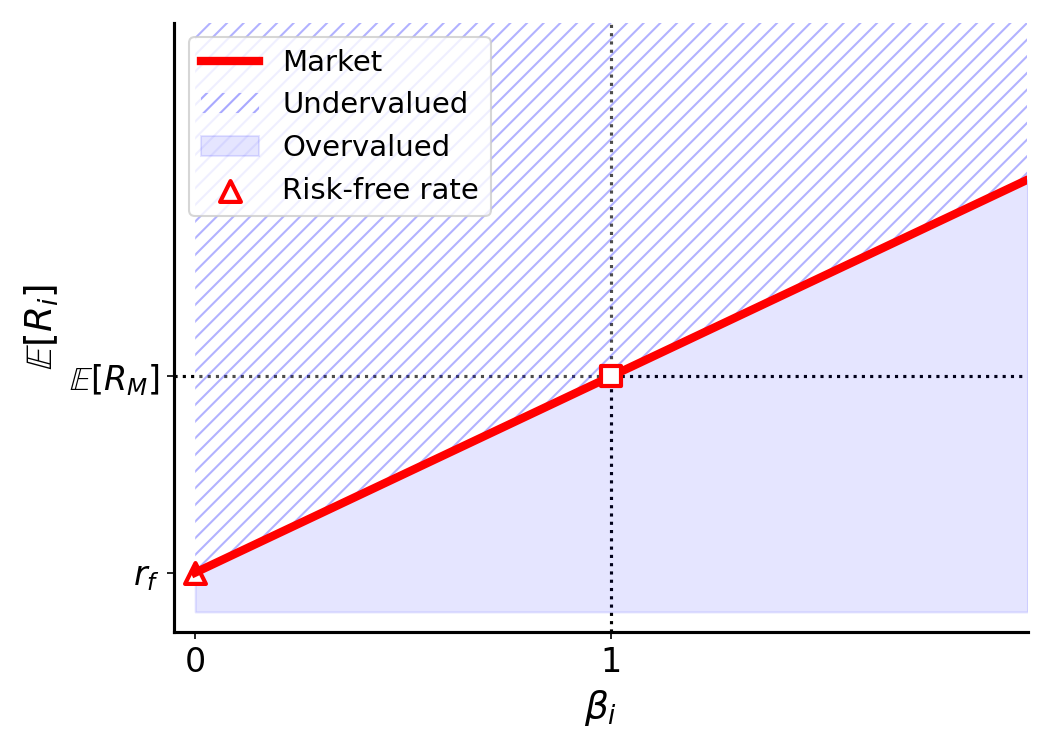
\includegraphics[width=0.6\textwidth]{LECTURE_4/SML.png}
    \caption{Security Market Line}
    \label{fig:security_market_line}
\end{figure}

\begin{example}
    Given the following market and company X data, estimate the expected stock return for company X:
    \begin{itemize}
        \item Market data
              \begin{itemize}
                  \item Risk-free rate: $2\%$
                  \item Expected market return: $8\%$
                  \item Market volatility: $10\%$
              \end{itemize}
        \item Company X data
              \begin{itemize}
                  \item Historical stock price return correlation to the market: $0.6$
                  \item Historical stock price volatility: $0.15$
              \end{itemize}
    \end{itemize}
    \textbf{Solution:}

    We can find the expected return of company X by:
    \begin{align*}
        \beta_i         & = \frac{\rho_{i,m} \sigma_i}{\sigma_{m}} = \frac{0.6 \cdot 0.15}{0.1} = 0.9 \\
        \mathbb{E}[R_i] & = r_f + \beta_i(\mathbb{E}[R_m] - r_f) = 0.02 + 0.9(0.08 - 0.02) = 0.074
    \end{align*}
\end{example}

\begin{definition}
    A company with a beta of 0.9 has a stock price that is currently trading at \$170 dollars a share. The current risk-free rate is 2\%, and the market rate is 7\%. What is the expected price of a share 5 years from now, if the company pays no dividends?\\

    \textbf{Solution:}

    We can find the expected return of the stock by:
    \begin{align*}
        \mathbb{E}[R_i] & = r_f + \beta_i(\mathbb{E}[R_m] - r_f) = 0.02 + 0.9(0.07 - 0.02) = 0.065        \\
        P_{t_0}         & = 170                                                                           \\
        P_{t_5}         & = P_{t_0} e^{r_{t_5} \cdot 5} = 170 e^{0.065 \cdot 5} = 170 e^{0.325} = \$235.3
    \end{align*}
\end{definition}


\begin{example}
    Consier a stock that has a current share price of \$10 and pays quarterly dividends of \$0.10 per share. Determine the expected stock price 3 years from now given the following:
    \begin{itemize}
        \item Expected market return: $10\%$
        \item Risk-free rate: $3\%$
        \item Company beta: $1.2$
    \end{itemize}

    \textbf{Solution:}

    We can find the expected return of the stock by:
    \begin{align*}
        \mathbb{E}[R_i] & = r_f + \beta_i(\mathbb{E}[R_m] - r_f) = 0.03 + 1.2(0.1 - 0.03) = 0.114
    \end{align*}
    We know that this gives us yearly effective compounding rate. We also want the quarterly compounding rate, per quarter:
    \begin{align*}
        (1 + 0.114)^{\frac{1}{4}} & = (1 + 0.114) \\
        r_{t_1}                   & = 0.02736
    \end{align*}
    Next we draw the cash-flow diagram for the stock:
    \begin{figure}[h!]
        \centering
        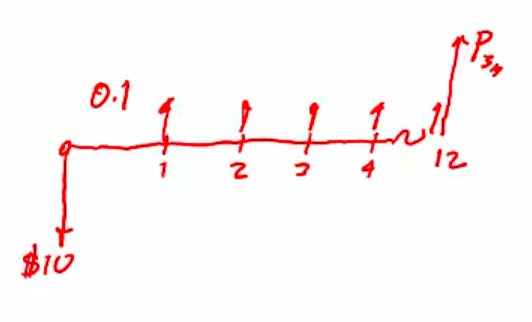
\includegraphics[width=0.6\textwidth]{LECTURE_4/cash-flow.png}
        \caption{Cash Flow Diagram}
        \label{fig:cash_flow_diagram}
    \end{figure}
    So we can model the diagram as:
    \begin{align*}
        P_0   & = \$0.1(P/A, 0.02736, 12) + P_3(P/F, 0.02736, 12) \\
        P_{3} & = \$ 12.43
    \end{align*}
\end{example}

\section{Arbitrage and Replicating Portfolio Diagrams}

\begin{definition}
    [Arbitrage]
    Arbitrage is the simultaneous purchase and sale of an asset to profit from a difference in the price. It is a trade that profits by exploiting the price differences of identical or similar financial instruments on different markets or in different forms.\\

    It occurs when there is an opportunity to achieve a risk-free gain at a rate of return that is higher than the risk-free rate.\\
\end{definition}

\begin{definition}
    [No Arbitrage Assumption (No Free Lunch)]
    The no-arbitrage assumption states that there are no risk-free profit opportunities in a perfect market.\\
\end{definition}


\begin{definition}
    [Forward/Futures Contract]
    A forward contract is a contract between two parties to buy or sell an asset at a specified future date at a price agreed upon today.\\

    A futures contract is the same, except it is traded on an exchange (thus, often less customized to any particular party).\\
\end{definition}

\begin{example}
    Say you could buy a bushel of corn for \$10 today and enter into a forward contract to deliver the corn for a pre-settled price of \$12 per bushel one year from now- assume it costs you nothing to store the corn. Say you could also borrow at 10\%.\\
    Is this an arbitrage opportunity?\\
    And what is the no-arbitrage price of corn (assuming the future price of corn is still \$12)?\\

    \textbf{Solution:}

    First we draw the cash-flow diagram for the situation:
    \begin{figure}[h!]
        \centering
        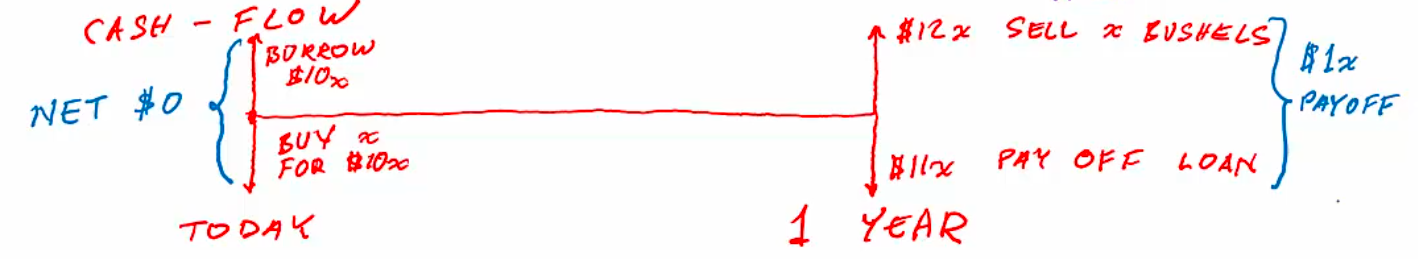
\includegraphics[width=0.6\textwidth]{LECTURE_4/cash-flow-2.png}
        \caption{Cash Flow Diagram}
        \label{fig:cash_flow_diagram_2}
    \end{figure}

    \begin{align*}
        F = +12 - 10(1+0.1) = 1
    \end{align*}
    So this is an arbitrage opportunity, because you can make a risk-free profit of \$1. In theory we should invest as much as possible in this opportunity, but in reality, laws of supply and demand will prevent this from happening.\\
    The no-arbitrage price of the forward contract can be found by:
    \begin{align*}
        P = \frac{12}{1+0.1} = \$10.91
    \end{align*}
    At this point there is no profit to be made.
\end{example}

\begin{example}
    Given an interest rate yield curve, determine the appropriate forward rate, $r_{t_1}$, that one could lock into today for specified interest rate from time $t_1$ to time $t_2$.\\
    \begin{figure}[h!]
        \centering
        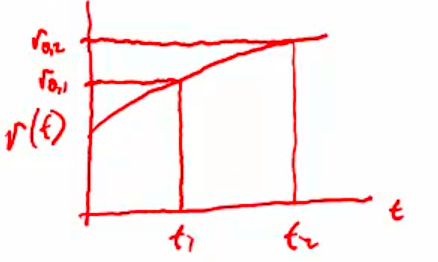
\includegraphics[width=0.6\textwidth]{LECTURE_4/interest-rate-curve.png}
        \caption{Interest Rate Curve}
        \label{fig:interest_rate_curve}
    \end{figure}

    \textbf{Solution:}

    We can use the \textbf{no-arbitrage assumption} to find two ways to get from $t_1$ to $t_2$ and equate them:
    \begin{align*}
        t = t_1 : \quad & F_1 = P_0e^{r_{0,1}t_1}                 \\
        t = t_2 : \quad & F_2 = F_1e^{r_{t_1,t_2}(t_2-t_1)}       \\
                        & F_2^{\prime} = F_1 e^{r_{1,2}(t_2-t_1)}
    \end{align*}
    The no-arbitrage assumption states that $F_2 = F_2^{\prime}$, so we can equate the two equations to find the forward rate:
    \begin{align*}
        F_2                                       & = F_2^{\prime}                          \\
        P_0e^{r_{0,1}t_1}e^{r_{t_1,t_2}(t_2-t_1)} & = P_0e^{r_{0,1}t_1}e^{r_{1,2}(t_2-t_1)} \\
        r_{1,2} = \frac{r_{0,1}t_1 + r_{t_1}}{t_2 - t_1}
    \end{align*}
\end{example}

\begin{example}
    [Using Replication to Price an Asset]
    \label{ex:replication}
    What is a fair price for a project whose payoff is \$140 if the market goes up and \$30 if the market goes down?\\
    \begin{itemize}
        \item The risk-free rate is 5\% for this period
        \item The current market portfolio is priced at \$100
        \item If the market goes up, it will be worth \$120
        \item If the market goes down, it will be worth \$95
    \end{itemize}
    If the probability of the market going up is 60\%, what is the expected return on the market portfolio? What is the expected return of the project?\\
    What if the expected payoff of the project was \$140, regardless of what the market did?\\

    \textbf{Solution:}

    The project can be modeled by the following diagram:


    \begin{figure}[h!]
        \centering
        \begin{subfigure}[b]{0.4\textwidth}
            \centering
            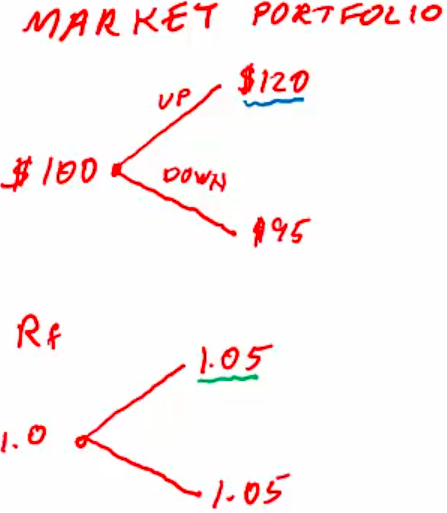
\includegraphics[width=\textwidth]{LECTURE_4/rep1.png}
            \caption{Market Portfolio Diagram}
            \label{fig:market_portfolio_diagram}
        \end{subfigure}
        \hfill
        \begin{subfigure}[b]{0.4\textwidth}
            \centering
            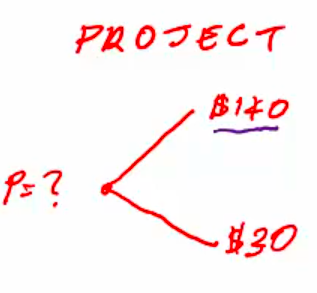
\includegraphics[width=\textwidth]{LECTURE_4/rep2.png}
            \caption{Project Diagram}
            \label{fig:project_diagram}
        \end{subfigure}

    \end{figure}
    We can solve for the for the factor $a, b$ that would make the project equivalent to the market portfolio:
    \begin{align*}
        \text{Up: }   & 140 = a \cdot 120 + b \cdot 1.05 \\
        \text{Down: } & 30 = a \cdot 95 + b \cdot 1.05
    \end{align*}
    Solving for $a, b$ gives us:
    \begin{align*}
        a & = 4.4    \\
        b & = -369.5
    \end{align*}
    So we can use this factors to find the present value of the project:
    \begin{align*}
        P_0 & = 4.4 \cdot 100 - 369.5 \cdot 1.00 = \$ 70.48
    \end{align*}
    Note: the probabilty of the market going up was not considered in this calculation.\\

\end{example}

\begin{definition}
    [Expected Value]
    The expected value of a project is the weighted average of the possible outcomes of the project, where the weights are the probabilities of the outcomes.\\
    \begin{equation}
        \mathbb{E}[P] = \sum_{i=1}^{n} P_i \cdot p_i
    \end{equation}
    Where:
    \begin{itemize}
        \item $P_i$ is the possible outcome of the project.
        \item $p_i$ is the probability of the outcome.
    \end{itemize}
\end{definition}

\begin{definition}
    [Expected Future Payoff/Return]

    The expected future payoff of the project is given by the expected value of the project, over the present value of the project:

    \begin{equation}
        \mathbb{E}[R] = \frac{\mathbb{E}[P]}{P_0} -1 = \frac{\sum_{i=1}^{n} P_i \cdot p_i}{P_0} -1
    \end{equation}

\end{definition}

\begin{example}
    Using the data from example \ref{ex:replication}, given that the probability of the market going up is $60\%$, what is the expected return of the market portfolio? What is the expected return of the project? And what is the systematic risk of the project?\\

    \textbf{Solution:}

    We can find the expected return of the market portfolio by:

    \begin{align*}
        \mathbb{E}[R_m] & = \frac{120\cdot 0.6 + 95\cdot 0.4}{100} - 1 = 0.1 = 10\%
    \end{align*}

    We can find the expected return of the project by:

    \begin{align*}
        \mathbb{E}[R_p] & = \frac{140\cdot 0.6 + 30\cdot 0.4}{70.48} - 1 = 36.2\%
    \end{align*}

    We can find the systematic risk of the project by:

    \begin{align*}
        \mathbb{E}[R_p] & = r_f + \beta_i(\mathbb{E}[R_m] - r_f) \\
        0.362           & = 0.05 + \beta_i(0.1 - 0.05)           \\
        \beta_i         & = 6.4
    \end{align*}
\end{example}

\begin{example}
    Again using the data from example \ref{ex:replication}, what would the present price be, given the expected payoff of the project was \$140, regardless of what the market did? And what would the present value be, if the project payoff was independent of the market, such that there was a 50\% chance of \$150, and a 50\% chance of \$130?\\

    \textbf{Solution:}

    This would mean the project is risk-free, and assuming no-arbitrage, we would simply discount to the present value using the risk-free rate (also, the systematic risk would be zero). So the present value of the project would be:
    \begin{align}
        P_0 & = \frac{140}{1.05} = \$133.33
    \end{align}

    We know $\beta = 0$, because there's no relation with the market conditions. So:
    \begin{align}
        \mathbb{E}[P] & = 150\cdot 0.5 + 130\cdot 0.5 = \$140 \\
    \end{align}
    And the present value of the project would be:
    \begin{align}
        P_0 & = \frac{140}{1.05} = \$133.33
    \end{align}

\end{example}


\begin{example}
    [Pricing an Asset with both Systematic and Idiosyncratic Risk]

    A wealthy (risk-neutral) investor has an opportunity to invest in a product development project. The outcome of the technology is uncertain, there is a 60\% chance that the technology works very well and a 40\% chance it will not meet all expectations. If the market goes up:
    \begin{itemize}
        \item And the technology works very well (60\% probability) the payoff will be \$80k
        \item Otherwise the payoff will be \$50k (technology did meet all expectations)
    \end{itemize}
    If the market goes down:
    \begin{itemize}
        \item And the technology works very well (60\% probability) the payoff will be \$55k
        \item Otherwise the payoff will be \$20k (technology did meet all expectations)
    \end{itemize}
    Other details include:
    \begin{itemize}
        \item Current market portfolio is \$45
        \item If the market goes up, payoff of the market portfolio will be \$60
        \item If the market goes down, payoff of the market portfolio will be \$40
        \item Risk-free rate is 5\%
        \item An initial investment of \$20k is required for the project
    \end{itemize}
    How much should the investor pay for the project?\\

    \textbf{Solution:}
    We can model the project with the following diagrams:

    \begin{figure}[h!]
        \centering
        \begin{subfigure}[b]{0.4\textwidth}
            \centering
            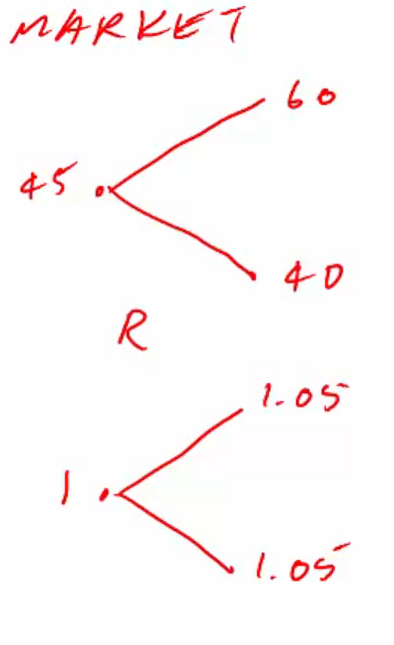
\includegraphics[width=\textwidth]{LECTURE_4/rep4.png}
            \caption{Market Portfolio Diagram}
            \label{fig:idiosyncratic_market_portfolio_diagram}
        \end{subfigure}
        \hfill
        \begin{subfigure}[b]{0.4\textwidth}
            \centering
            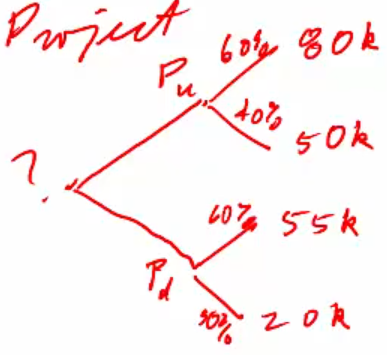
\includegraphics[width=\textwidth]{LECTURE_4/rep3.png}
            \caption{Project Diagram}
            \label{fig:idiosyncratic_project_diagram}
        \end{subfigure}

    \end{figure}

    We can first solve for the expected values of the project if the market goes up and down:
    \begin{align*}
        \mathbb{E}[P] & = \$80k \cdot 0.6 + \$50k \cdot 0.4 = \$68k \\
        \mathbb{E}[P] & = \$55k \cdot 0.6 + \$20k \cdot 0.4 = \$41k
    \end{align*}
    Now we can solve for $a, b$ that would make the project equivalent to the market portfolio:

    \begin{align*}
        \text{Up: }   & \$68k = a \cdot 60 + b \cdot 1.05 \\
        \text{Down: } & \$41k = a \cdot 40 + b \cdot 1.05
    \end{align*}

    Solving for $a, b$ gives us:
    \begin{align*}
        a & = 1.35k    \\
        b & = -12.38 k
    \end{align*}

    So we can use this factors to find the present value of the project:

    \begin{align*}
        P_0 & = 1.35 \cdot 45 - 12.38 \cdot 1.00 = \$48.37k
    \end{align*}
    But since there's a $20k$ initial investment, the investor should pay:
    \begin{align*}
        P_0 = \$48.37k - \$20k = \$28.37k
    \end{align*}
\end{example}

· A company is looking to issue a 5 year bond with a coupon rate of 5%
paid annually
· You have determined that the $risk-neutral$ probability of a company
defaulting on the bond in any given year is 5% and in the case of a default
only half of the principal will be paid out
· What should be the price of the bond if the risk-free rate is 3%?
· What is the yield rate?

\begin{example}
    [Pricing a Bond with Default Risk]
    A company is looking to issue a 5 year bond with a coupon rate of 5\% paid annually. You have determined that the risk-neutral probability of a company defaulting on the bond in any given year is 5\% and in the case of a default only half of the principal will be paid out.
    \begin{itemize}
        \item What is the probability of the company not defaulting in any given year?
        \item What should be the price of the bond if the risk-free rate is 3\%?
        \item What is the yield rate?
    \end{itemize}

    \textbf{Solution:}

    We can find the probability of the company not defaulting in any given year by:
    \begin{align*}
        \text{Probability of never defaulting: } 0.95^5 & = 0.77378 \\
        \text{Probability of defaulting: } 1 - 0.77378  & = 0.22622
    \end{align*}

    We can find the price of the bond by drawing the replicating portfolio diagram:
    \begin{figure}
        \centering
        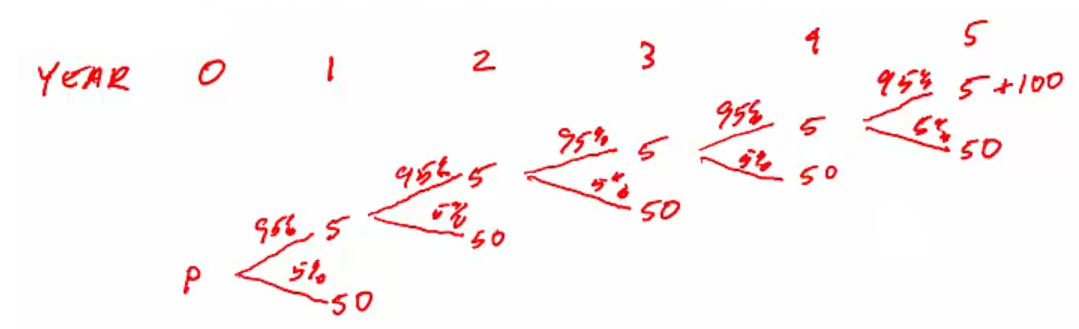
\includegraphics[width=0.6\textwidth]{LECTURE_4/rep5.png}
        \caption{Replicating Portfolio Diagram}
        \label{fig:replicating_portfolio_diagram}
    \end{figure}

    We start from the end and work our way back to find the price of the bond:
    \begin{align*}
        P_{up}^{(4)}   & = 5 + \frac{\mathbb{E}[P^{(5)}]}{1.03} & = 5 + \frac{105\times0.95 + 50.5\times0.05}{1.03} = 104.27 \\
        P_{down}^{(4)} & = 50
    \end{align*}
    Above gives the price at year 4, right when we receive the coupon/payout. We can now find the price at year 3:
    \begin{align}
        P_{up}^{(3)}   & = 5 + \frac{\mathbb{E}[P^{(4)}]}{1.03} & = 5 + \frac{104.27\times0.95 + 50\times0.05}{1.03} = 103.6 \\
        P_{down}^{(3)} & = 50                                                                                                \\
        P_{up}^{(2)}   & = 5 + \frac{\mathbb{E}[P^{(3)}]}{1.03} & = 5 + \frac{103.6\times0.95 + 50\times0.05}{1.03} = 102.41 \\
        P_{down}^{(2)} & = 50                                                                                                \\
    \end{align}
    We can now find the price at year 1, remember, we don't receive a coupon at year 1:
    \begin{align*}
        P_{up}^{(1)} & = \frac{\mathbb{E}[P^{(2)}]}{1.03} & = \frac{102.41\times0.95 + 50\times0.05}{1.03} = 96.88
    \end{align*}

    The yield can be found by:
    \begin{align*}
        P                & = A(P/A, i_{\text{yield}}, N) + F(P/F, i_{\text{yield}}, N) \\
        96.88 = 5(P/A, i_{\text{yield}}, 5) + 100(P/F, i_{\text{yield}}, 5)            \\
        i_{\text{yield}} & = 0.05735
    \end{align*}
\end{example}

% \chapter{Comparison Methods 1}

\section{Project Relationships and alternatives}

\begin{definition}
    [Independent Projects]
    Expected costs and benefit of each project \underline{do not depend} on whether or not the other is chosen.\\
    E.g. Painting a room and building a fence are two independent projects.
\end{definition}

\begin{definition}
    [Mutually Exclusive Projects]
    Only one of the possible projects can be chosen.\\
    E.g. You want to buy one car, so choosing one car means you can't choose the others.
\end{definition}

\begin{remark}
    Your budget can be the difference between projects being independent or mutually exclusive. If you can't afford both, then they are mutually exclusive.
\end{remark}

\begin{definition}
    [Related but not Mutually Exclusive Projects]
    Projects that are not independent but not mutually exclusive.\\
    E.g. Spending on one project may reduce the amount you can invest in another.
\end{definition}

\begin{theorem}
    [Converting Related Projects to Mutually Exclusive Projects]
    If you have many related projects, then you can form mutually exclusive options by choosing a combination of projects in each scenario
\end{theorem}

\section{Present Worth and Annual Worth}

\begin{remark}
    Motivation: When evaluating projects, what discount rate do we use to compare cash-flows at different times?
\end{remark}

\subsection{Present Worth}

\begin{definition}
    [MARR (Minimum Attractive Rate of Return)]
    Intuition: If I don't invest in this project, what can I expect to earn from the best alternative? So, not taking a project means, you'll be earning at the MARR.
\end{definition}

\begin{definition}
    [Present Worth (PW), or Net Present Value (NPV)]
    The present value of benefits (positive cash-flows) minus the present value of costs (negative cash-flows), discounted at the MARR.\\
    Intuition: The amount by which the project beats the best alternative, expressed as today's value
\end{definition}

\begin{proposition}
    [Independent Projects Evaluation with PW]
    \begin{align}
        PW > 0 & \implies \text{Accept the project} \\
        PW < 0 & \implies \text{Reject the project}
    \end{align}
\end{proposition}

\subsection{Annual Worth}

\begin{definition}
    [Annual Worth (AW)]
    Annual Worth is the equivalent annuity of the present worth. It is the constant annual cash-flow that has the same present worth as the project.
\end{definition}

\begin{proposition}
    [Independent Projects Evaluation with AW]
    \begin{align}
        AW > 0 & \implies \text{Accept the project} \\
        AW < 0 & \implies \text{Reject the project}
    \end{align}
\end{proposition}

\begin{remark}
    So we solve for an annuity for annual worth, and a present value for present worth.
\end{remark}

\section{Evaluating Mutually Exclusive Projects (PW and AW)}

\begin{theorem}
    [Evaluating Mutually Exclusive Projects with PW]
    \begin{itemize}
        \item[]
        \item Define the time horizon
        \item Develop hte cash flows for each alternative
        \item Calculate the PW for each alternative using MARR
        \item Compare the PWs and pick the alternative with the highest PW
        \item[] \begin{itemize}
                  \item The best alternative may be none if all PWs are negative
              \end{itemize}
    \end{itemize}
\end{theorem}

\begin{definition}
    [Time Horizon]
    The time horizon is the time period over which the project is evaluated. It is the time period over which the cash flows are calculated.\\
    This is usually the life of the investment.
\end{definition}

\subsection{Normalizing Time Horizons}

\begin{theorem}
    [Repeated Lives]
    When comparing projects with different time horizons, we can assume that at the end of each project's life, the project is repeated (purchased again). This occurs for the Lowest Common Multiple of the time horizons.
\end{theorem}
\begin{remark}
    When using annual worth, we don't need to normalize time horizons.
\end{remark}

\begin{theorem}
    [Study Period]
    We assume we can terminate the project that lasts longer so it matches the shorter project's time horizon, and we adjust the salvage value to account for the remaining life of the longer project.
\end{theorem}

% \chapter{Comparison Methods 2}

\section{Internal Rate of Return (IRR)}

\begin{remark}
    Intuition: Cash-flow methods requires a discount rate for comparison, these methods find what the inherit rate of return for a project is.
\end{remark}

\begin{definition}
    [Internal Rate of Return (IRR)]
    The IRR is the discount rate that makes the present worth of the benefits equal to the present worth of the costs.\\
    Intuition: The rate of return that the project earns.
\end{definition}

\begin{theorem}
    [Finding IRR]
    Using a cash-flow diagram, find the discount rate that makes the PW equal to zero.
\end{theorem}

\begin{figure}[H]
    \centering
    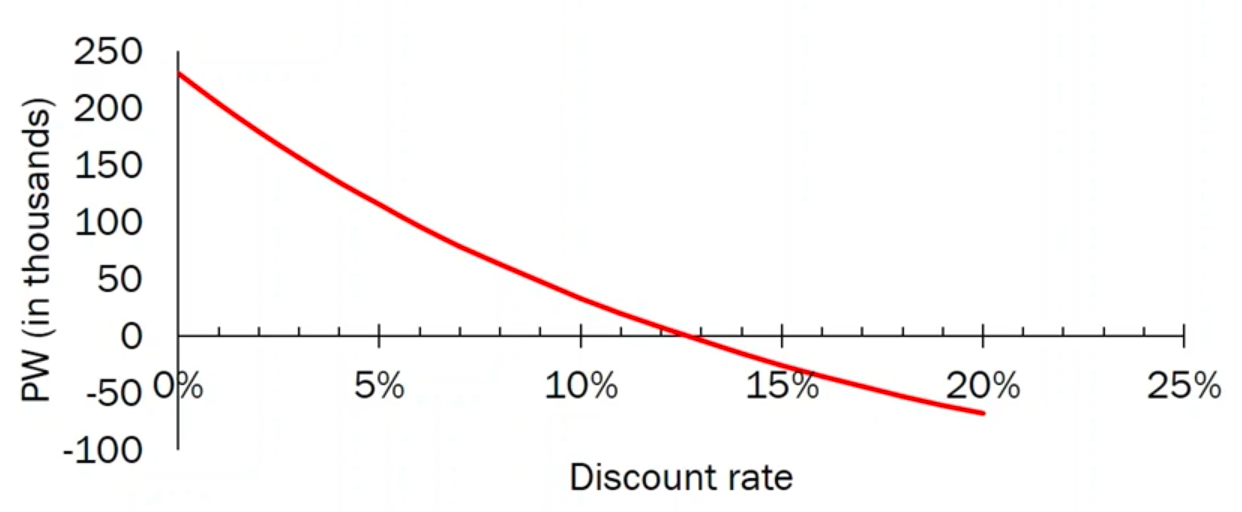
\includegraphics[width=0.5\textwidth]{LECTURE_6/IRR.png}
    \caption{PW vs. Discount Rate Graph for a Simple Project}
\end{figure}

\begin{proposition}
    [Evaluating Simple Projects with IRR]

    \textbf{Where the investment is simple} (i.e. all negative cash-flows precede positive cash-flows):
    \begin{itemize}
        \item If $IRR > MARR$, accept the project
        \item If $IRR < MARR$, reject the project
    \end{itemize}
\end{proposition}

\begin{proposition}
    [Limitations of IRR]
    When the investment is not simple, there will be two solutions to the equation that satisfies the PW = 0. In this case, it may not a good measure of the project's profitability.
\end{proposition}

\begin{figure}[H]
    \centering
    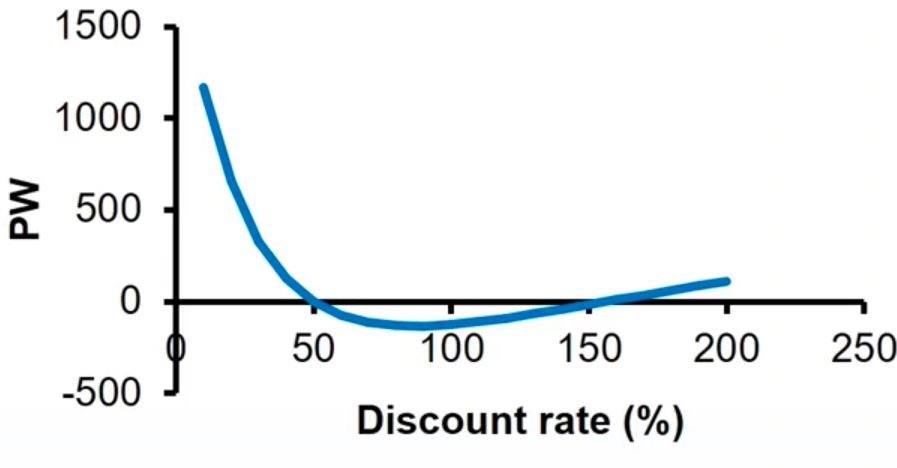
\includegraphics[width=0.5\textwidth]{LECTURE_6/not-simple.png}
    \caption{PW vs. Discount Rate Graph for a Complex Project}
\end{figure}

\section{Payback Period}


\begin{definition}
    [Payback Period]
    The payback period is the time it takes for the project to recover the initial investment.
\end{definition}

\begin{theorem}
    [Finding Payback Period]
    Using a cash-flow diagram, find the time it takes for the cumulative cash-flow to reach zero (not discounted).
\end{theorem}

\begin{theorem}
    [Discounted Payback Period]
    The discounted payback period is the time it takes for the \underline{discounted} cumulative cash-flow, the Present Worth, to reach zero.
\end{theorem}

\begin{proposition}
    [Evaluation of the Payback Period Method]
    \begin{itemize}
        \item Answers "When will I make my money back?"
        \item Easy to use/understand, \textbf{especially if the investment was not meant to make money}
        \item Not a sound method in Engineering Economics and against its principles
        \item[] \begin{itemize}
                  \item Ignores the cash-flows after the payback period, so it can overlook long-term investments
              \end{itemize}
    \end{itemize}
\end{proposition}

\section{Comparing Mutually Exclusive Projects Using IRR}

\begin{proposition}
    [IRR for Mutually Exclusive Projects]
    IRR can be misleading when comparing mutually exclusive projects. Take the following example:\\
    You can invest in the bank for a rate of return of $10\%$, or in the following projects:
    \begin{itemize}
        \item Lend your friend \$10 for a return of \$15 in 1 year (IRR = $50\%$)
        \item Lend your friend \$20 for a return of \$28 in 1 year (IRR = $40\%$)
    \end{itemize}
    The IRR method would suggest that you should lend your friend \$10 but consider that investing \$10 in your friend and \$10 in the bank would yield $10\cdot 1.1 + 10\cdot 1.5 = 26$ which is less than $\$20\cdot 1.4 = 28$, so you should invest in the second project. \\
    \textbf{Therefore, the IRR can mislead when the size of the investment is not considered.}
\end{proposition}
\begin{theorem}
    [Incremental IRR]
    This solves the problem of comparing mutually exclusive projects by comparing increments between two projects.\\
    \begin{itemize}
        \item Order alternatives in increasing order of first costs
        \item Start with the 'do nothing' alternative
        \item Calculate the IRR of the first alternative, if it is greater than the MARR, keep this as the best option so far
        \item Calculate the iterative IRR of the next alternative compared to the previous best option
        \item When comparing two alternatives, get the $\Delta FC$ (difference in first costs) and $\Delta A$ (difference in annual benefits) and solve for $PW =0$ to get the IRR
    \end{itemize}
\end{theorem}



\end{document}